\documentclass{anstrans}
\usepackage{amsmath}
\usepackage{amssymb}
%\usepackage{amsthm}
\usepackage{amscd}
%\usepackage{amsfonts}
\usepackage{graphicx}%
\usepackage{fancyhdr}
\usepackage{color}
\usepackage{cite}

%\usepackage[T1]{fontenc}
%\usepackage[utf8]{inputenc}
%\usepackage{authblk}
\usepackage{physics}
\usepackage{float}
\usepackage{caption}
\usepackage{subcaption}

\setlength{\columnsep}{0.5 in}

\newcommand{\expv}[1]{\ensuremath{\mathbb{E}[ #1]}}
\newcommand{\xs}[2]{\ensuremath{\Sigma_{#1}^{(#2)}}}
\newcommand{\intO}{\ensuremath{\int\limits_{4\pi}}}
\newcommand{\intz}{\ensuremath{\int\limits_0^1}}
\newcommand{\intf}{\ensuremath{\int\limits_{-\infty}^\infty}}
\newcommand{\intzf}{\ensuremath{\int\limits_{0}^\infty}}
\newcommand{\LargerCdot}{\raisebox{-0.25ex}{\scalebox{1.2}{$\cdot$}}}

%\textwidth6.6in
%\textheight9in


%\setlength{\topmargin}{0.3in} \addtolength{\topmargin}{-\headheight}
%\addtolength{\topmargin}{-\headsep}

%\setlength{\oddsidemargin}{0in}

%\oddsidemargin  0.0in \evensidemargin 0.0in \parindent0em

%\pagestyle{fancy}\lhead{MATH 579 (UQ for PDEs)} \rhead{02/24/2014}
%\chead{Project Proposal} \lfoot{} \rfoot{\bf \thepage} \cfoot{}
\title{Sparse-Grid Stochastic Collocation Uncertainty Quantification Convergence for Multigroup Diffusion}

\author{Paul W. Talbot, Anil K. Prinja}
\institute{Department of Nuclear Engineering, University of New Mexico, Albuquerque, NM, 87131}
\email{talbotp@unm.edu \and prinja@unm.edu}
%\date{}


\begin{document}
\section{Introduction}
Advanced methods in  uncertainty quantification for numerical models in computational physics \cite{SCLagrange}\cite{textbook} are gaining widespread acceptance in nuclear modeling \cite{erin01}\cite{mike01}.  However, little attention has been paid to the convergence rates of these methods in stochastic space.  We demonstrate the efficiency of sparse-grid stochastic collocation \cite{sparseSC} in comparison with analog Monte Carlo for uncertainty quantification through convergence studies.

%\subsection{Problem}
The physical system we consider is a two-dimensional quarter-core reactor, consisting of 5 materials distributed in 121 regions (see Fig. \ref{geom}).  We solve the two-group neutron diffusion criticality approximation
\begin{align}
-\grad\cdot\qty( D_1(\bar x)\grad\phi_1(\bar x))+&\qty(\xs{a}{1}(\bar x)+\xs{s}{1\to2}(\bar x))\phi_1(\bar x) \nonumber\\
        &= \frac{1}{k(\phi)}\sum_{g'=1}^2\nu_{g'}\xs{f}{g'}(\bar x)\phi_{g'}(\bar x),
\end{align}
\begin{equation}
-\grad \cdot\qty(D_2(\bar x)\grad \phi_2(\bar x))+\xs{a}{2}(\bar x)\phi_2(\bar x) = \xs{s}{1\to 2}(\bar x)\phi_1(\bar x).
\end{equation}
We apply vacuum boundaries on the top and right, and reflecting boundaries on the bottom and left.
The criticality eigenvalue and quantity of interest $k(\phi)$ is given by
\begin{equation}
k(\phi)=\sum_{g=1}^2\iint\limits_D\frac{\nu\xs{f}{g}\phi_g(\bar x)}{\qty(-\nabla\cdot D_g\nabla+\Sigma_r^{(g)})\phi_g(\bar x)}~d\bar x.
\end{equation}
The material properties are shown in Table \ref{tab:coremats}, and the domain $\Omega=[0,200\text{ cm}]^2$.  The reference value $k$=1.00007605445.
\begin{figure}[H]
\centering
  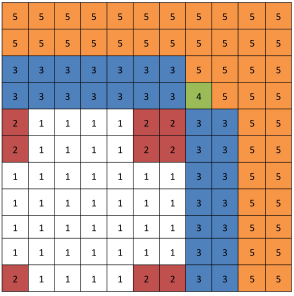
\includegraphics[width=0.5\linewidth]{core}
  \caption{Core Geometry}
  \label{geom}
\end{figure}
\begin{table}[h]
\centering
\begin{tabular}{c c | c c c c}
Mat. & $g$ & $D_g$ & $\Sigma_{a,g}$ & $\nu\Sigma_{f,g}$ & $\Sigma_s^{1,2}$ \\ \hline
1 & 1 & 1.255 & 8.252e-3 & 4.602e-3 & 2.533e-2 \\
 & 2 & 2.11e-1 & 1.003e-1 & 1.091e-1 & \\ \hline
2 & 1 & 1.268 & 7.181e-3 & 4.609e-3 & 2.767e-2 \\
 & 2 & 1.902e-1 & 7.047e-2 & 8.675e-2 & \\ \hline
3 & 1 & 1.259 & 8.002e-3 & 4.663e-3 & 2.617e-2 \\
 & 2 & 2.091e-1 & 8.344e-2 & 1.021e-1 & \\ \hline
4 & 1 & 1.259 & 8.002e-3 & 4.663e-3 & 2.617e-2 \\
 & 2 & 2.091e-1 & 7.3324e-2 & 1.021e-1 & \\ \hline
5 & 1 & 1.257 & 6.034e-4 & 0 & 4.754e-2 \\
 & 2 & 1.592e-1 & 1.911e-2 & 0 & 
\end{tabular}
\caption{Reference Material Properties for Benchmark Core}
\label{tab:coremats}
\end{table}
%\begin{figure}[H]
%\centering
%  \begin{subfigure}[b]{0.2 \textwidth}
%   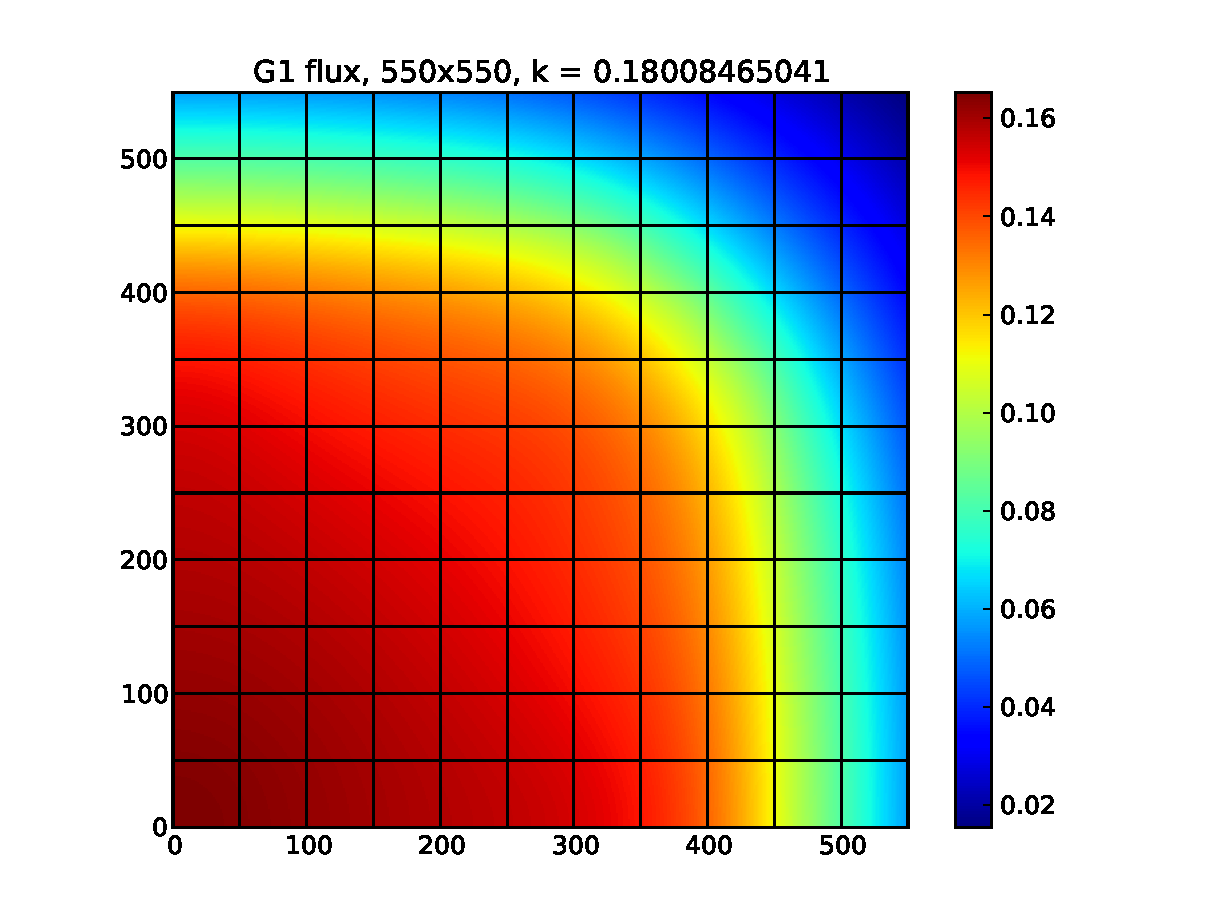
\includegraphics[width=\textwidth]{g1_50_flux}
%   \caption{$\phi$, Group 1}
%   \label{g1}
%  \end{subfigure}
%  \begin{subfigure}[b]{0.2 \textwidth}
%   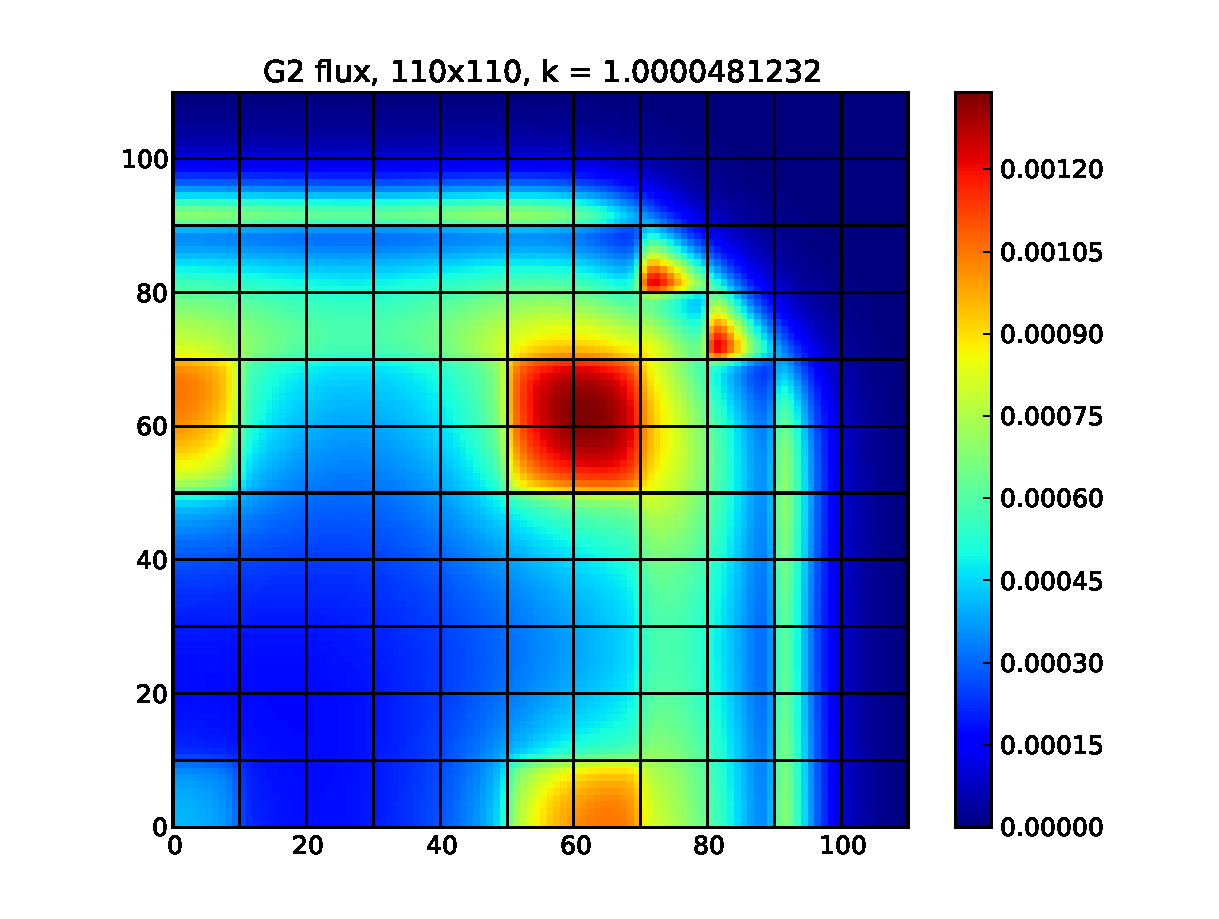
\includegraphics[width=\textwidth]{g2_50_flux}
%   \caption{$\phi$, Group 2}
%   \label{g2}
%  \end{subfigure}
%  \caption{Reference Flux Profiles}
%  \label{benchflux}
%\end{figure}

%\begin{figure}[H]
%  \centering
%   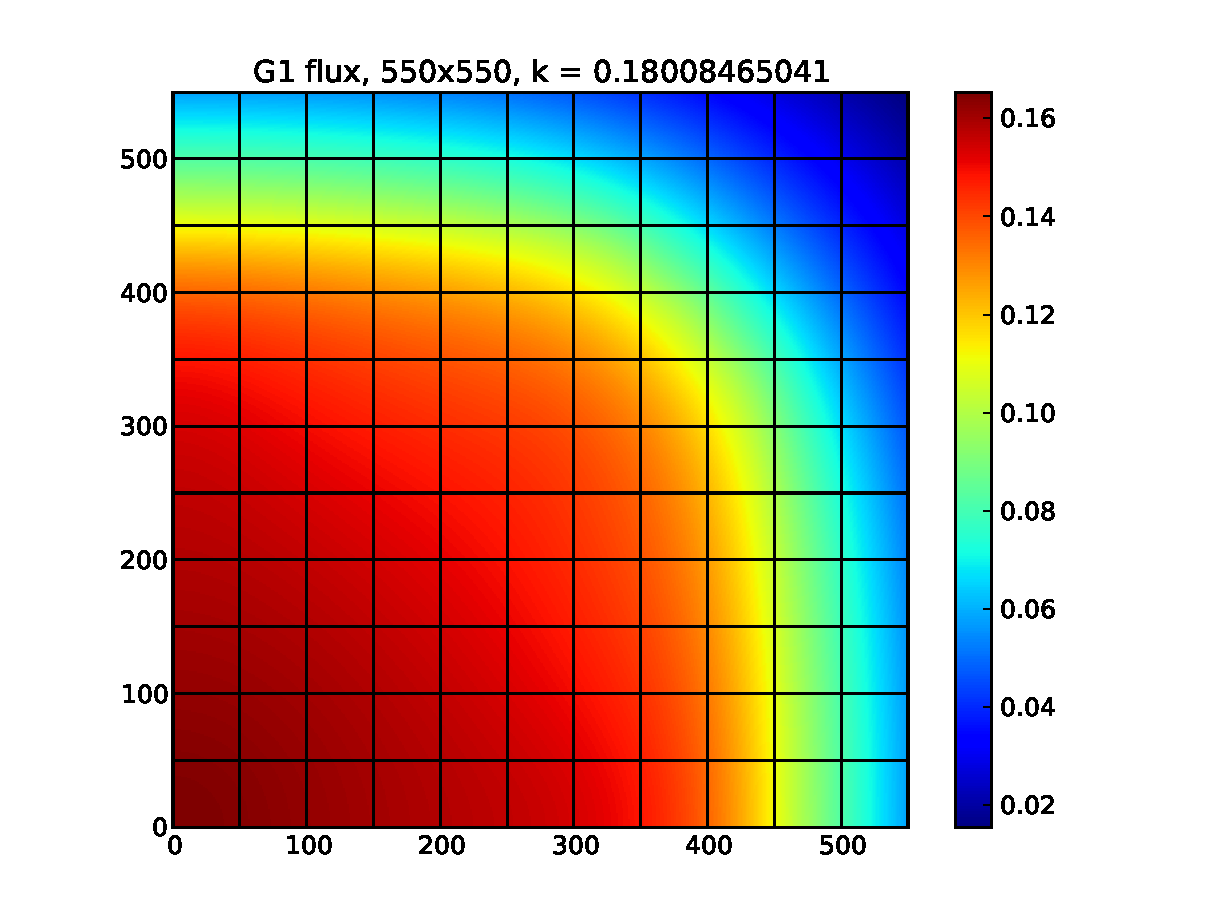
\includegraphics[width=0.45\textwidth]{g1_50_flux}
%   \caption{Reference Flux $\phi$, Group 1}
%   \label{g1}
%\end{figure}
%\begin{figure}[H]
%  \centering
%   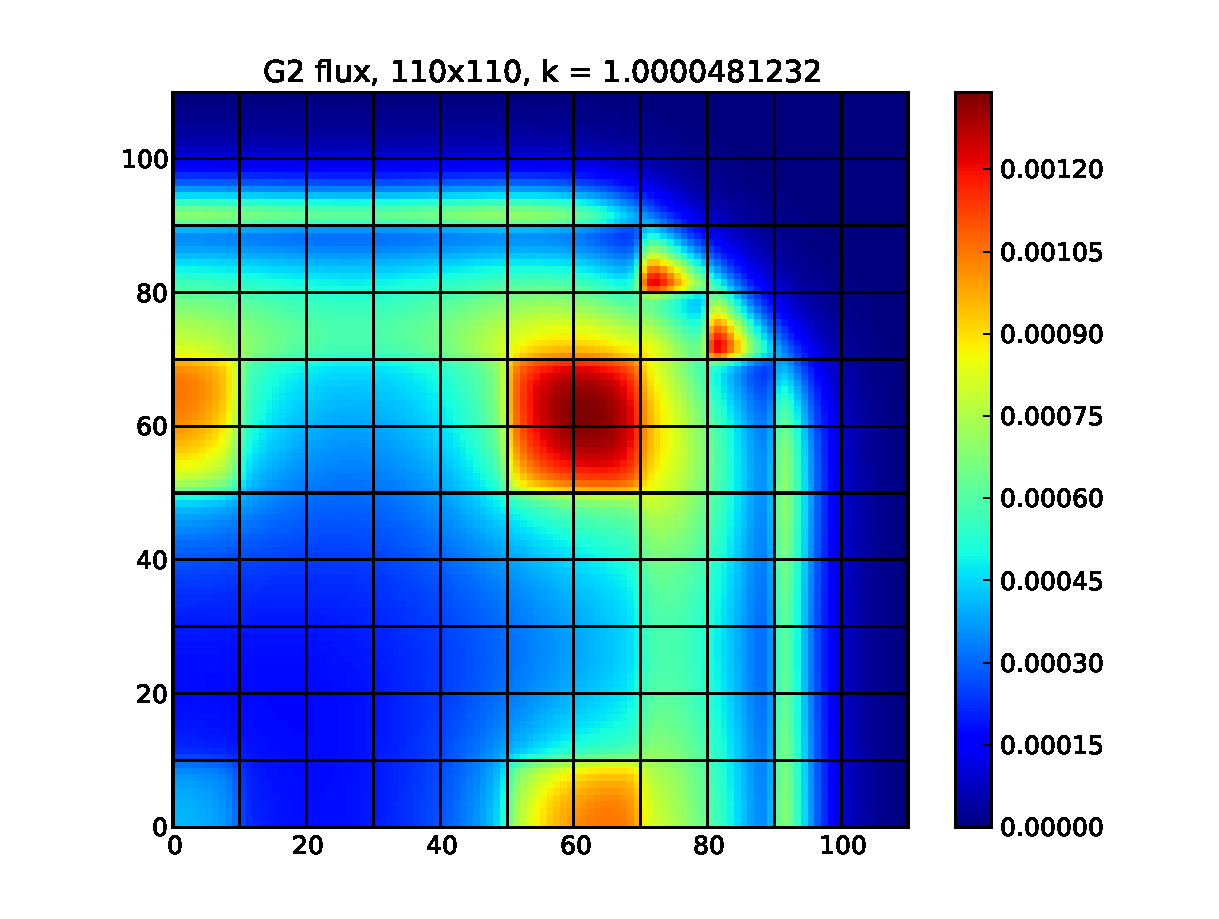
\includegraphics[width=0.45\textwidth]{g2_50_flux}
%   \caption{Reference Flux $\phi$, Group 2}
%   \label{g2}
%\end{figure}

%\subsection{Stochastic Problem}
The material cross sections, neutron multiplication factors, and diffusion coefficients are potential uncertain input parameters.  We introduce uniformly-distributed uncertainty within 10\% of the reference values.  The uncertain distributions make up the uncertainty space $\Gamma\subset\mathbb{R}^N,$ where $N$ is the number of uncertain parameters.  While we always use all 5 materials in the problem, we allow uncertainty in only $N$ input parameters.  We consider the input parameter uncertainties to be independently distributed.

\section{Methods}
%\subsection{Deterministic Space}
We solve our system of equations by imposing a mesh grid on the physical domain using the local and global particle-conserving finite volume method.  We solve the system of equations nonlinearly with the criticality eigenvalue, using Jacobian-free Newton-Krylov methods.  We use the GMRES algorithm in the \texttt{trilinos} solver package.% from Sandia National Laboratory \cite{Trilinos-Overview}.  

%\subsection{Stochastic Space}
Our primary interest in this study is evaluating the practicality of using stochastic collocation on sparse grids \cite{sparse1}\cite{sparse2}\cite{sparseSC} to quantify uncertainty in diffusion problems. We use analog Monte Carlo uncertainty quantification as a benchmark, and a high-resolution solution for the moments of $k$ in stochastic space as a reference solution. We compare Monte Carlo and stochastic collocation solutions to the reference as a function of the number of transport solves to contrast convergence rates. 

In stochastic solves, we treat the deterministic transport solver non-intrusively as a functional of the uncertain input parameters.  To avoid confusion in labels, we will represent $k(Y)$ by a more generic $u(Y)$, where $Y\in\Gamma$ is the vector of uncertain inputs.
%\subsubsection{Monte Carlo}
In Monte Carlo uncertainty quantification, the uncertain vector $Y$ is randomly sampled $M$ times, and moments are derived from the solution realizations.  For example, 
\begin{equation}
\expv{u(Y)} = \int_\Gamma u(Y) \rho(Y) dY\approx \frac{1}{M}\sum_{m=1}^M u(Y_m),
\end{equation}
\begin{equation}
\expv{u(Y)^2} = \int_\Gamma u(Y)^2 \rho(Y) dY\approx \frac{1}{M}\sum_{m=1}^M u(Y_m)^2,
\end{equation}
where each $Y_m$ is a single realization randomly sampled from the domain of $Y$.

%\subsubsection{Stochastic Collocation}
In stochastic collocation for sparse grids, we approximate $u(Y)$ as the sum of the product of $u$ evaluated at $\eta$ collocated points and multidimensional Lagrangian polynomials.  Using $k$ as the quadrature index,
\begin{equation}\label{approx}
u(Y)\approx u_{h,\eta,\Lambda(L)}(Y)=\sum_{k=0}^\eta u(Y^{(k)})\mathcal{L}_k(Y),
\end{equation}
\begin{equation}
\mathcal{L}_k(Y)=\prod_{n=1}^N \mathcal{L}_{k_n}(Y_n),
\end{equation}
\begin{equation}
\mathcal{L}_{k_n}(Y_n)=\prod_{j=1}^i \frac{Y_n-Y_n^{(i)}}{Y_n^{(k_n)}-Y_n^{(i)}},
\end{equation}
\begin{equation}
\expv{u(Y)}\approx\expv{u_h(Y)}=\sum_{k=1}^\eta w_k ~u_h\qty(Y^{(k)}),
\end{equation}
where $u_h(Y)$ is the spatially-discretized PDE solution, and $Y^{(k)}=[Y^{(k_1)},\cdots,Y^{(k_N)}]$ are realizations of $Y$ chosen at quadrature points $Y^{(k)}$ with corresponding weights $w_k$.  We use Gauss-Legendre quadrature to obtain collocation points and weights.  The order of the quadrature is obtained based on polynomial expansion orders from an index set $\Lambda(L)$.  For a single uncertain parameter ($N=1$) and a fourth-order polynomial approximation ($L=4$), $\Lambda$ includes all polynomial orders from 0 to 4 $\qty(\Lambda=[0,1,2,3,4])$.  Each index point $p\in\Lambda$ corresponds to a polynomial expansion moment of order $p$.

There are several methods to determine multivariate $\Lambda$.
The most naive case is a tensor product $\Lambda_\text{TP}(L)$ of polynomial expansion orders,
\begin{equation}
\Lambda_\text{TP}(L)=\Big\{\bar p=[p_1,...,p_N]: \max_{1\leq n\leq N}p_n\leq L \Big\}.%\hspace{5pt}|\Lambda_\text{TP}(L)|=(L+1)^2.\nonumber
\end{equation}
Other index sets with less cardinality can be employed to reduce the number of collocation points and counteract the $\Lambda_\text{TP}$ curse of dimensionality.  We consider the \emph{total degree} ($\Lambda_\text{TD}$) set, which is ideal for quantities that are analytic in stochastic space; and the \emph{hyberbolic cross} ($\Lambda_\text{HC}$) index set for quantities that have finite smoothness in stochastic space,
\begin{equation}
\Lambda_\text{TD}(L)=\Big\{\bar p=[p_1,...,p_N]:\sum_{n=1}^N p_n \leq L \Big\},%|\Lambda_\text{TD}(L)|={L+N\choose N},
\end{equation}
\begin{equation}
\Lambda_\text{HC}(L)=\Big\{\bar p=[p_1,...,p_N]:\prod_{n=1}^N p_n+1 \leq L+1 \Big\}.
\end{equation}
%\begin{equation}
%|\Lambda_\text{HC}(L)|\leq (L+1)(1+\log(L+1))^{N-1}.
%\end{equation}
%Figure \ref{indexsets} shows each of these index sets for $N=2,L=4$.  
%\begin{figure}[H]
%\centering
%  \begin{subfigure}[b]{0.15 \textwidth}
%   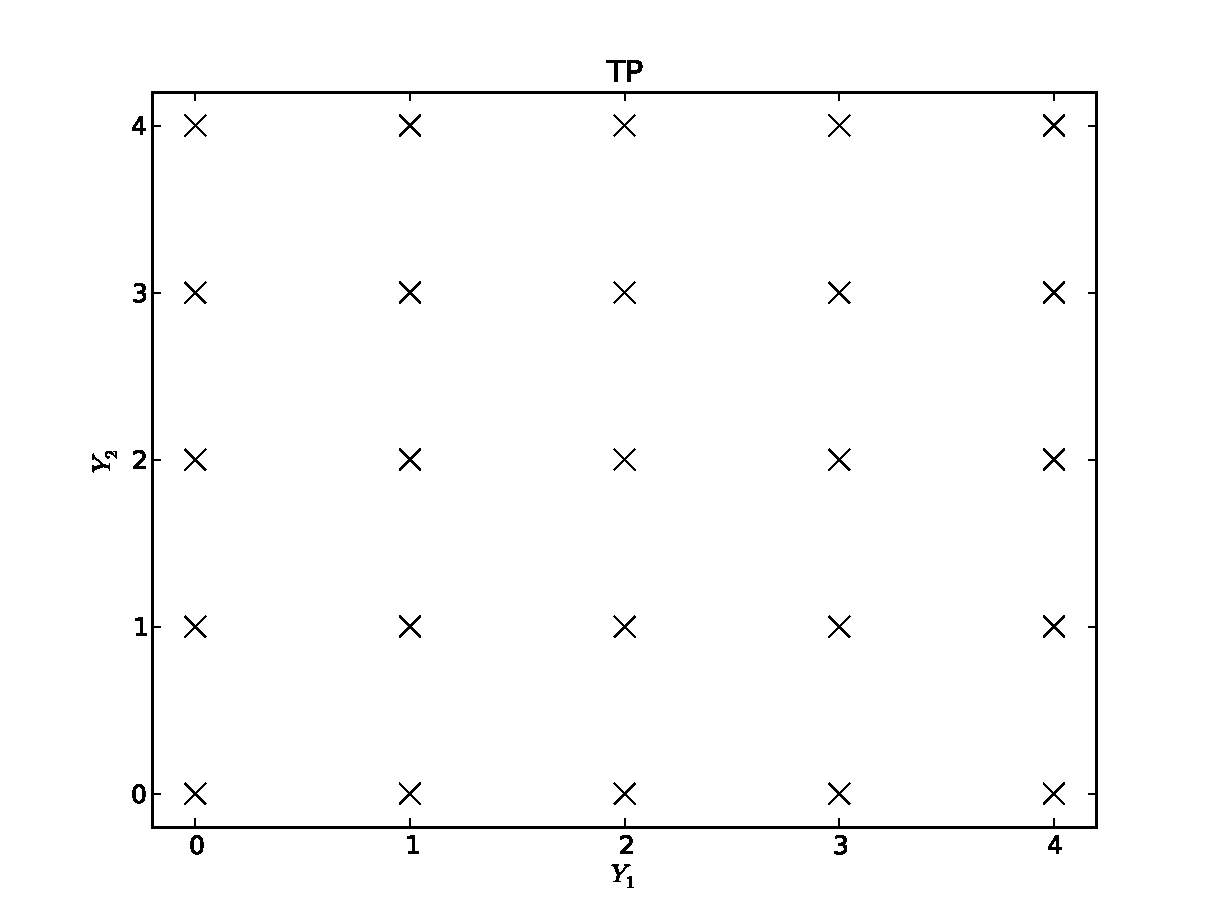
\includegraphics[width=\textwidth]{TP}
%   \caption{Tensor Product}
%   \label{TP}
%  \end{subfigure}
%  \begin{subfigure}[b]{0.15 \textwidth}
%   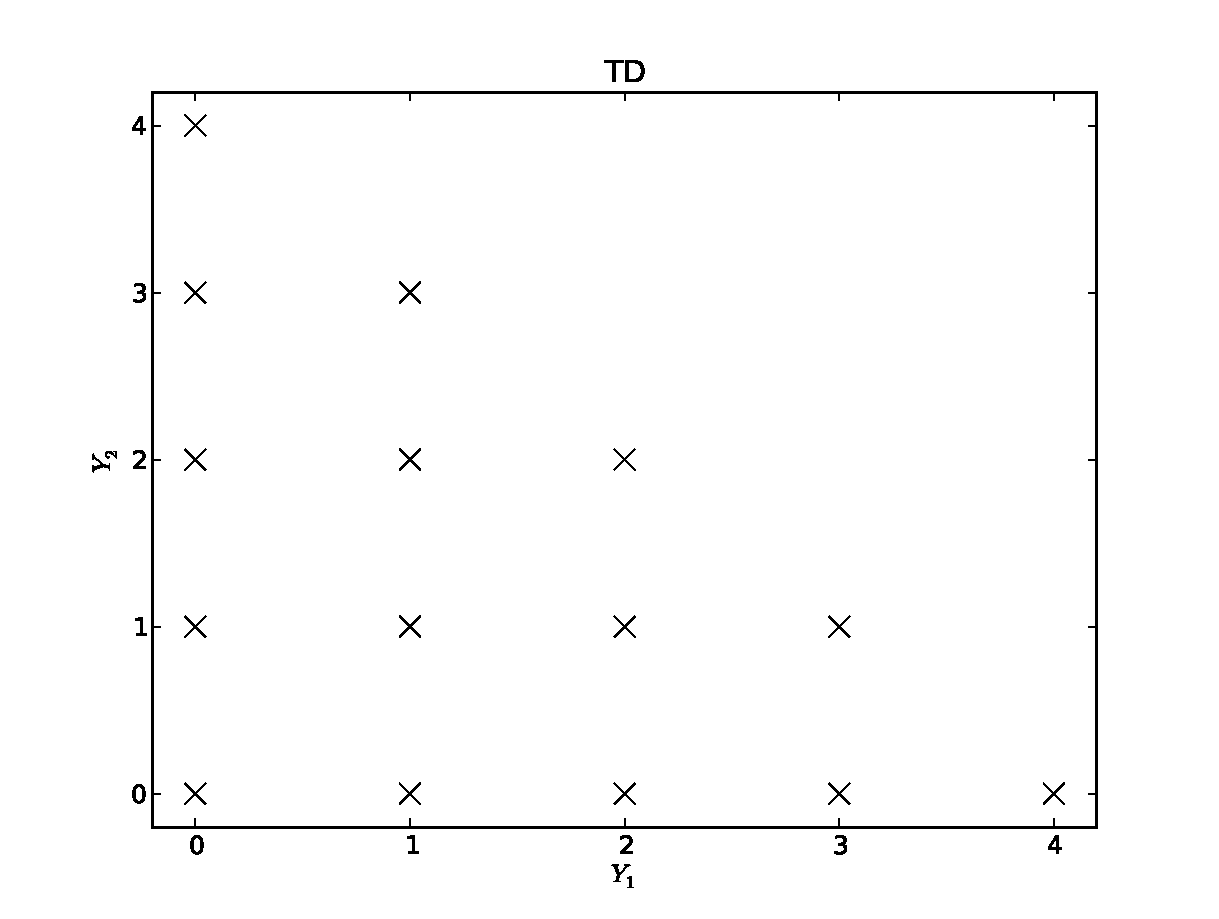
\includegraphics[width=\textwidth]{TD}
%   \caption{Total Degree}
%   \label{TD}
%  \end{subfigure}
%  \begin{subfigure}[b]{0.15 \textwidth}
%   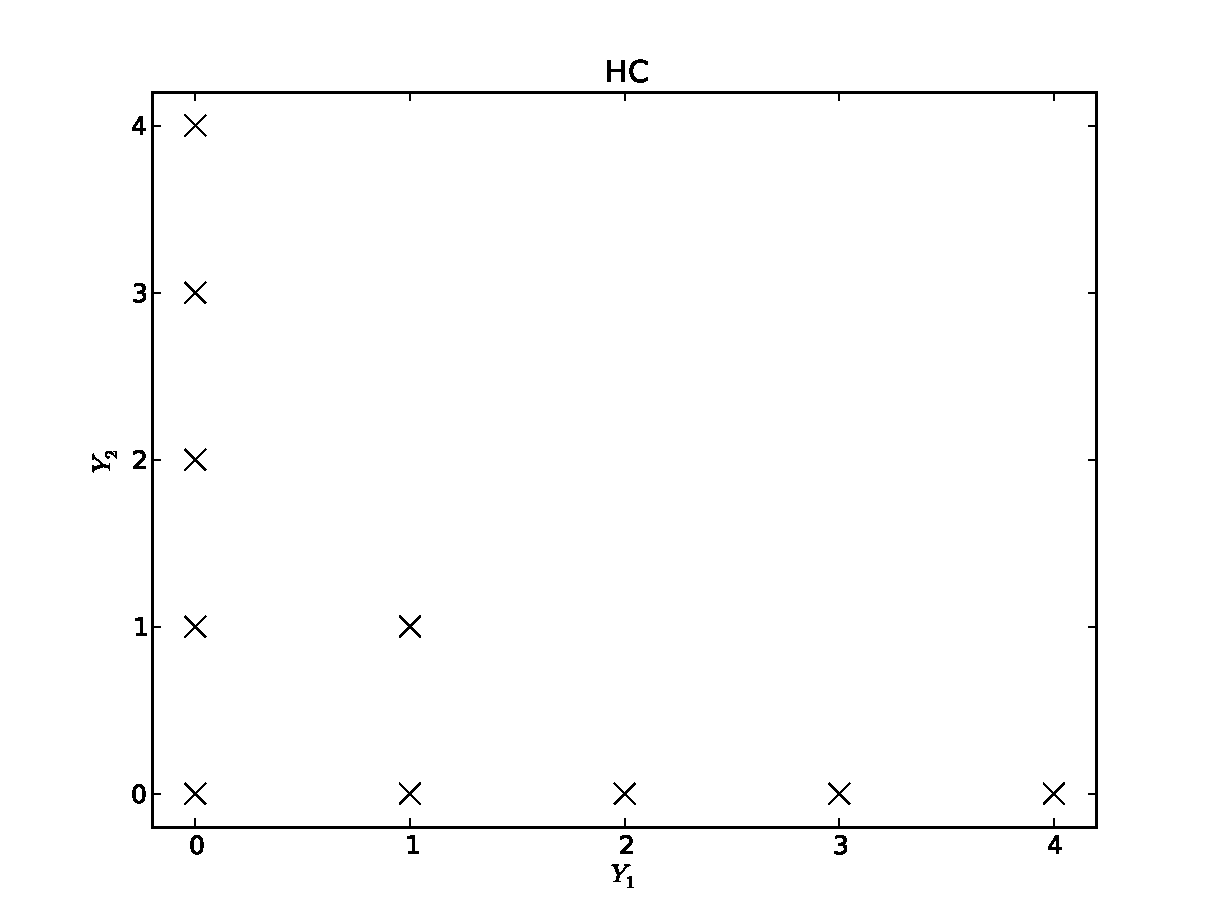
\includegraphics[width=\textwidth]{HC}
%   \caption{Hyperbolic Cross}
%   \label{HC}
%  \end{subfigure}
%  \caption{Index Set Examples: $N=2,L=4$}
%  \label{indexsets}
%\end{figure}
%
%\begin{figure}[h]
%  \centering
%   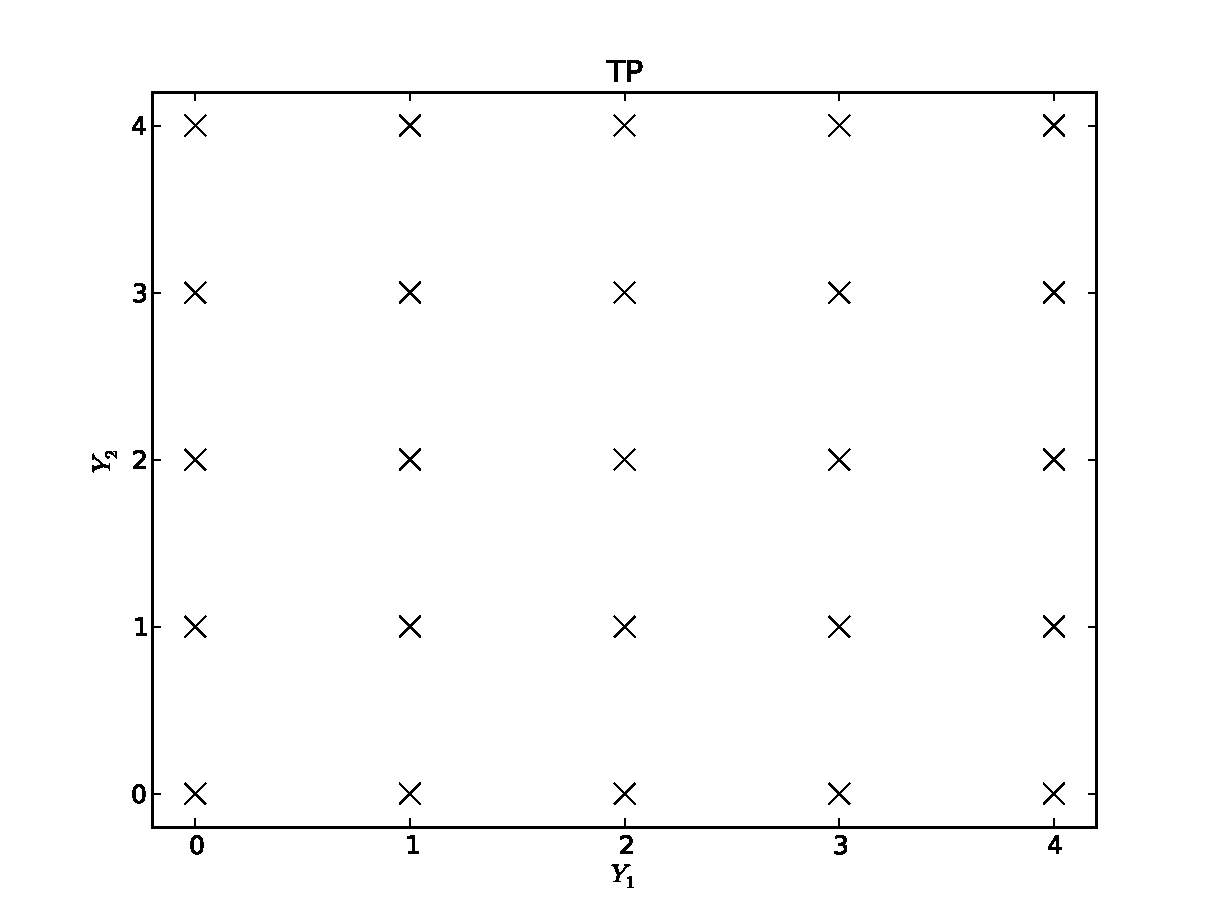
\includegraphics[width=0.45\textwidth]{TP}
%   \caption{Tensor Product}
%   \label{TP}
%\end{figure}
%\begin{figure}[h]
%  \centering
%   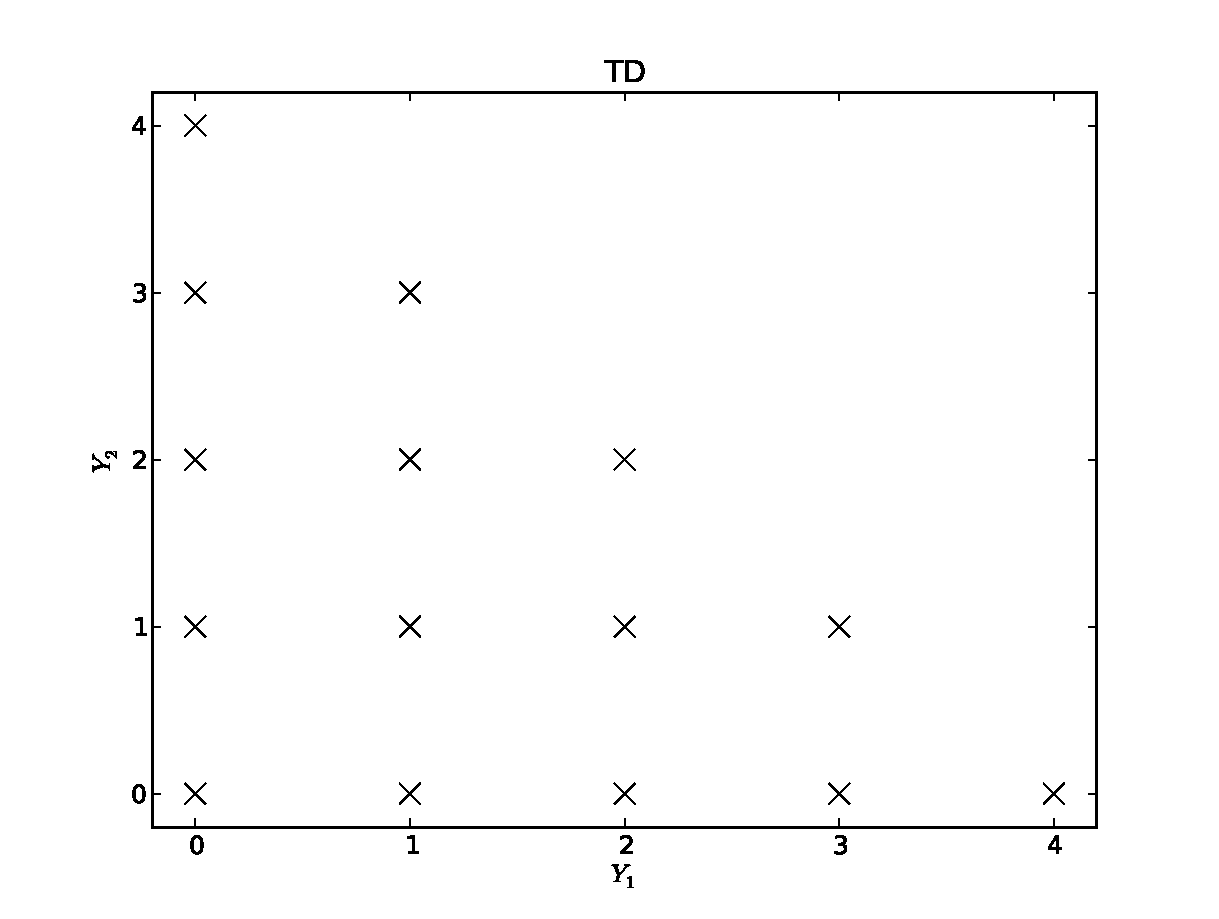
\includegraphics[width=0.45\textwidth]{TD}
%   \caption{Total Degree}
%   \label{TD}
%\end{figure}
%\begin{figure}[h]
%  \centering
%   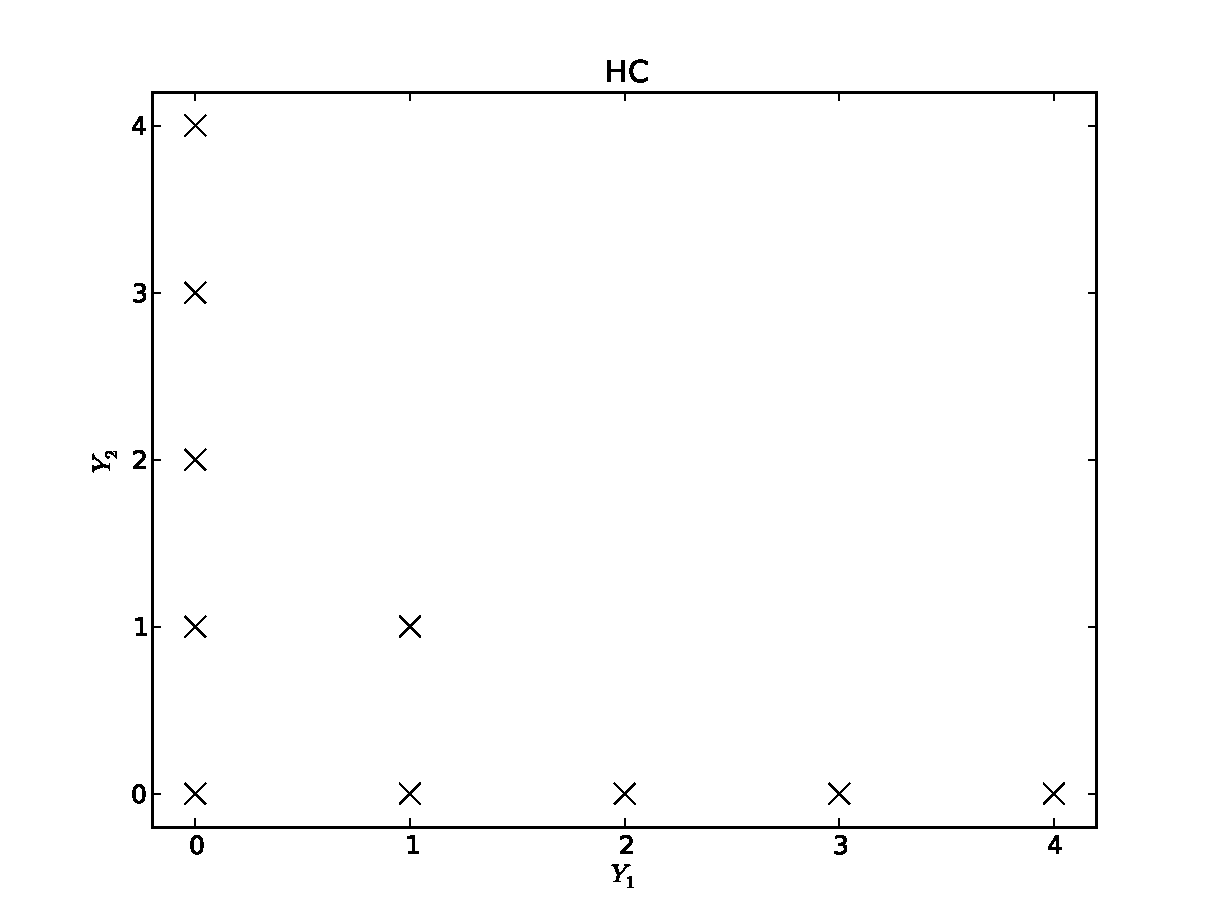
\includegraphics[width=0.45\textwidth]{HC}
%   \caption{Hyperbolic Cross}
%   \label{HC}
%\end{figure}

%\begin{figure}[H]
%\centering
%  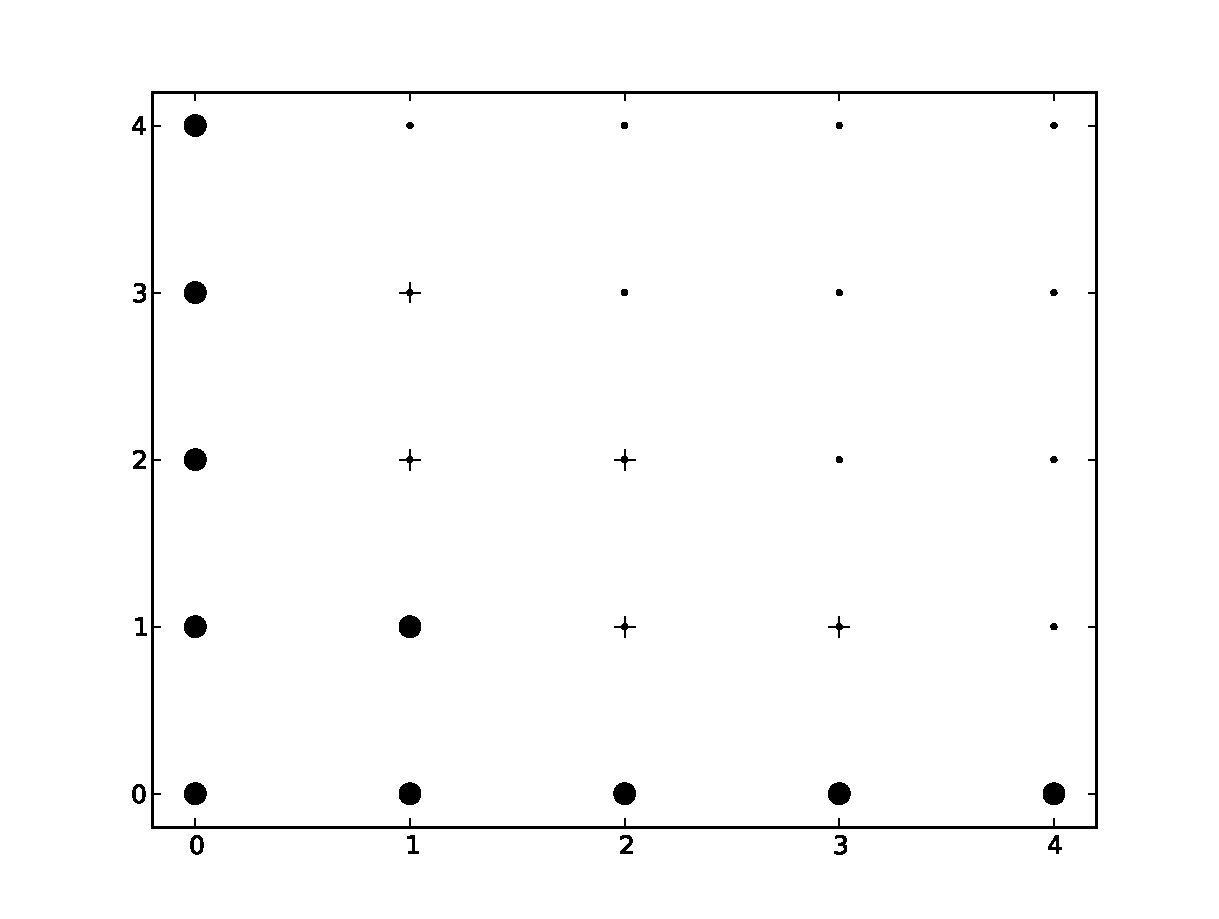
\includegraphics[width=0.5\linewidth]{indexsets}
%  \caption{Index Sets ($\cdot$ TP, + TD, $\bullet$ HC) }
%  \label{indexsets}
%\end{figure}


The collocation points used in the Lagrange polynomial expansion are obtained based on the index set chosen.
This provides the isotropic sparse grid approximation
\begin{equation}
k(Y)\approx\mathcal{S}_{N,\Lambda(L)}[k](Y)=\sum_{\boldsymbol{i}\in\Lambda(L)}c(\boldsymbol{i})\bigotimes_{n=1}^N\mathcal{U}_{n,p(i_n)}[u](Y),
\end{equation}
\begin{equation}
c(\boldsymbol{i})=\sum_{\substack{\boldsymbol{j}=\{0,1\}^N,\\ \boldsymbol{i}+\boldsymbol{j}\in\Lambda(L)}}(-1)^{|\boldsymbol{j}|_1},
\end{equation}
\begin{equation}
\bigotimes_{n=1}^N\mathcal{U}_{n,p(i_n)}[u](Y)\equiv\sum_{k}^{p(\vec i)}u_h\qty(Y^{(k)})\mathcal{L}_k(Y),
\end{equation}
where we use $p(i)=i$ as the \emph{quadrature rule} used to obtain the number of quadrature points for a polynomial expansion order.
The reduction in collocation points due to sparse grids improves with the number of input parameters $N$ and the expansion order $L$.  
%For comparison, we show the number of index points for two input spaces of dimensionality $N$ and several expansion levels $L$ for all three index sets, as well as the number of collocation points for total degree and hyperbolic cross rules in Table \ref{compIS}.  We note that accuracy cannot be directly drawn from polynomial expansions; as shown in Section \ref{results}, for this problem the same number of collocation points results in a similar magnitude error in both total degree and hyperbolic cross.  This implies, for this problem, that a much lower-order polynomial expansion constructed using the total degree rule is comparable in error to a larger-order polynomial expansion constructed using the hyperbolic cross rule.
%\begin{figure}[H]
%\centering
  %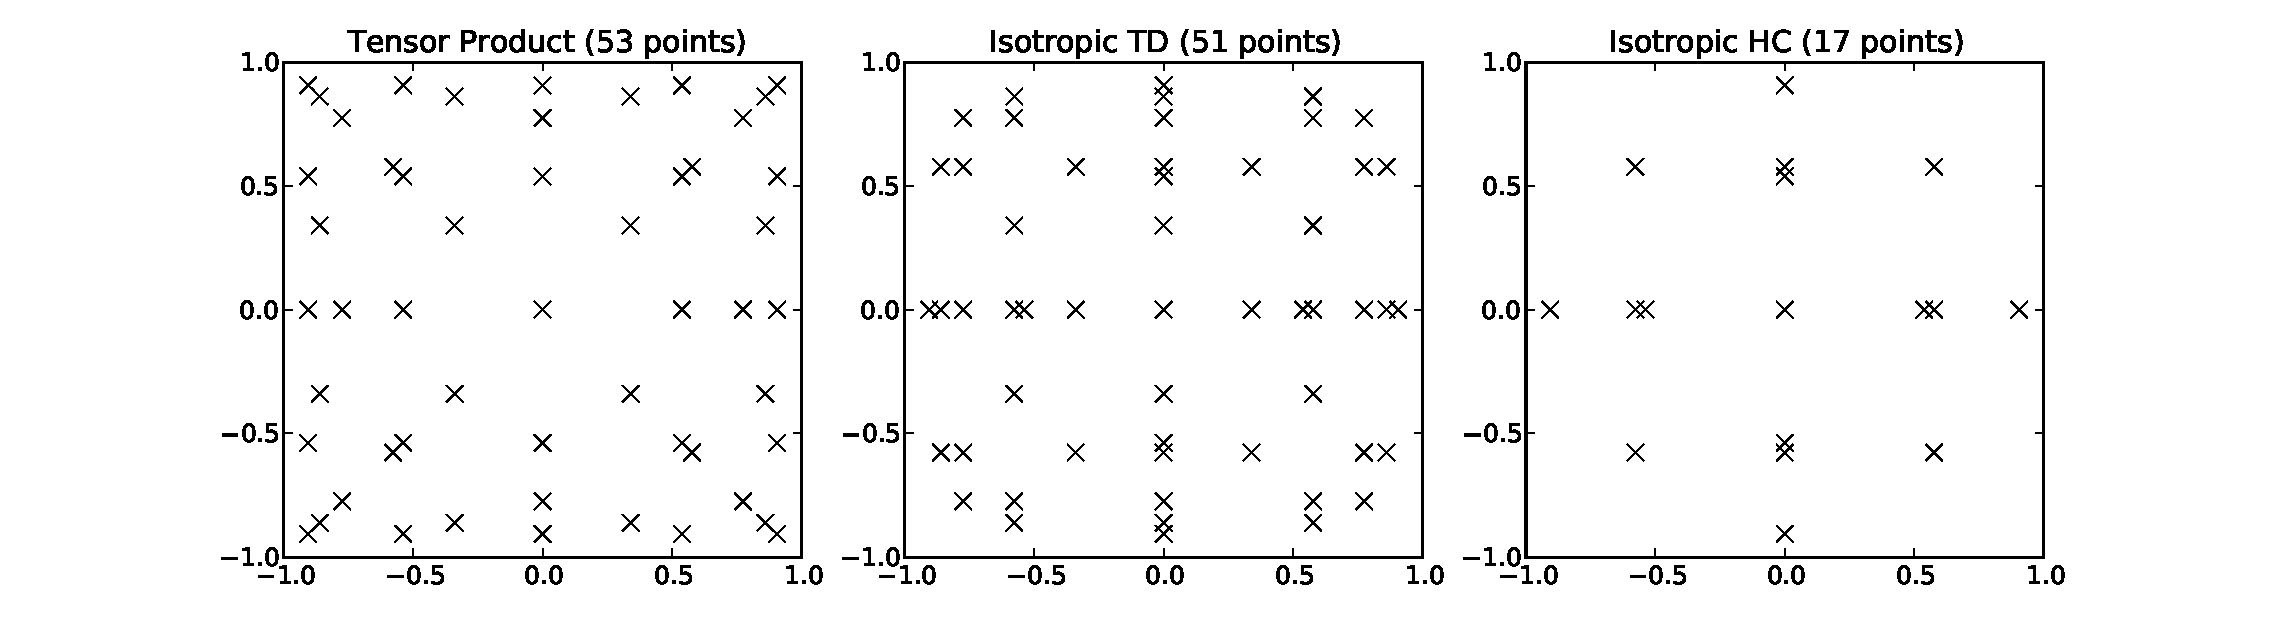
\includegraphics[width=\linewidth]{sparse_plot}
  %\caption{Sparse Grids, $N=2,L=4,p(i)=i$, Legendre points}
 % \label{collsets}
%\end{figure}
%\begin{table}
%\centering
%\begin{tabular}{c|c|c|c c|c c}
%$N$ & $L$ & TP & \multicolumn{2}{|c|}{TD} & \multicolumn{2}{|c}{HC} \\ 
%$N$ & $L$ & $\qty|\Lambda(L)|$ & $\qty|\Lambda(L)|$ & $\eta$ & $\qty|\Lambda(L)|$ & $\eta$\\ \hline
%3 & 4 & 125    & 35    & 165   & 16 & 31\\
% & 8   & 729    & 165  & 2,097  & 44 & 153\\
% & 16 & 4,913  & 969   & 41,857 & 113 & 513\\
% & 32 & 35,737 & 6,545 & 1,089,713 & 309 & 2,181\\ \hline
%5 & 2 & 293 & 21 & 61 & 11 & 11\\
% & 4 & 3,125 & 126 & 781 & 31 & 71\\
% & 8 & 59,049 & 1,287 & 28,553 & 111 & 481 
%\end{tabular}
%\caption{Index Set and Collocation Size Comparison}
%\label{compIS}
%\end{table}
%While the hyberbolic cross collocation points are significantly more sparse than the total degree collocation points, we note that the increased number of polynomial expansion moments in total degree make it much more accurate for the same total polynomial expansion level $L$.  The results of this work demonstrate that for this problem, the same number of collocation points using either total degree or hyperbolic cross results in a similar magnitude of error.

\subsubsection{Anisotropic Sparse Grids}
In many cases, the sensitivity of the stochastic solution to one uncertain dimension is less than another.  %For example, we heuristically expect the sensitivity of the $k$-eigenvalue to the reflecting material (material 5) diffusion coefficient to be much less than the sensitivity to the fission cross section in the main fissile material (material 1).  
We introduce importance coefficients $\vec\alpha=[\alpha_1,\cdots,\alpha_N]$ that parametrize the sensitivity of the stochastic solution to each uncertain input.  Using the one-norm
%\begin{equation}
$\qty|\vec\alpha|_1\equiv\frac{1}{N}\sum_{n=1}^N \alpha_n,$
%\end{equation}
these weight parameters adjust the index set rules $\Lambda(L)$ for total degree and hyperbolic cross as
\begin{equation}
\tilde\Lambda_\text{TD}(L)=\Big\{\bar p=[p_1,...,p_N]:\sum_{n=1}^N \alpha_n p_n \leq \qty|\vec\alpha|_1 L \Big\},
\end{equation}
\begin{equation}
\tilde\Lambda_\text{HC}(L)=\Big\{\bar p=[p_1,...,p_N]:\prod_{n=1}^N \qty(p_n+1)^{\alpha_n} \leq \qty(L+1)^{\qty|\vec\alpha|_1} \Big\}.
\end{equation}
Smaller values of $\alpha_n$ are assigned to more sensitive dimensions to prioritize collocation points.

\section{Results}\label{results}
%\subsection{Deterministic Convergence}
%In Figs. \ref{spatialphi}-\ref{spatialk} we demonstrate the physical convergence of the deterministic PDE solver as we refine the spatial mesh grid.  Both fluxes as well as the $k$-eigenvalue converge between first and second order.  The finite volume method is second order, but the overall convergence order is reduced by first-order boundary condition treatments.  In all cases, reducing the size of $h=\Delta x=\Delta y$ decreases the error to a fine solution.  The reference solution is one level of refinement finer than the finest point shown.   The flux error is calculated by considering the maximum error among several pointwise flux values, while $k$ error is the global value for each refinement.
%\begin{figure}[H]
%\centering
%  \begin{subfigure}[b]{0.45 \textwidth}
%   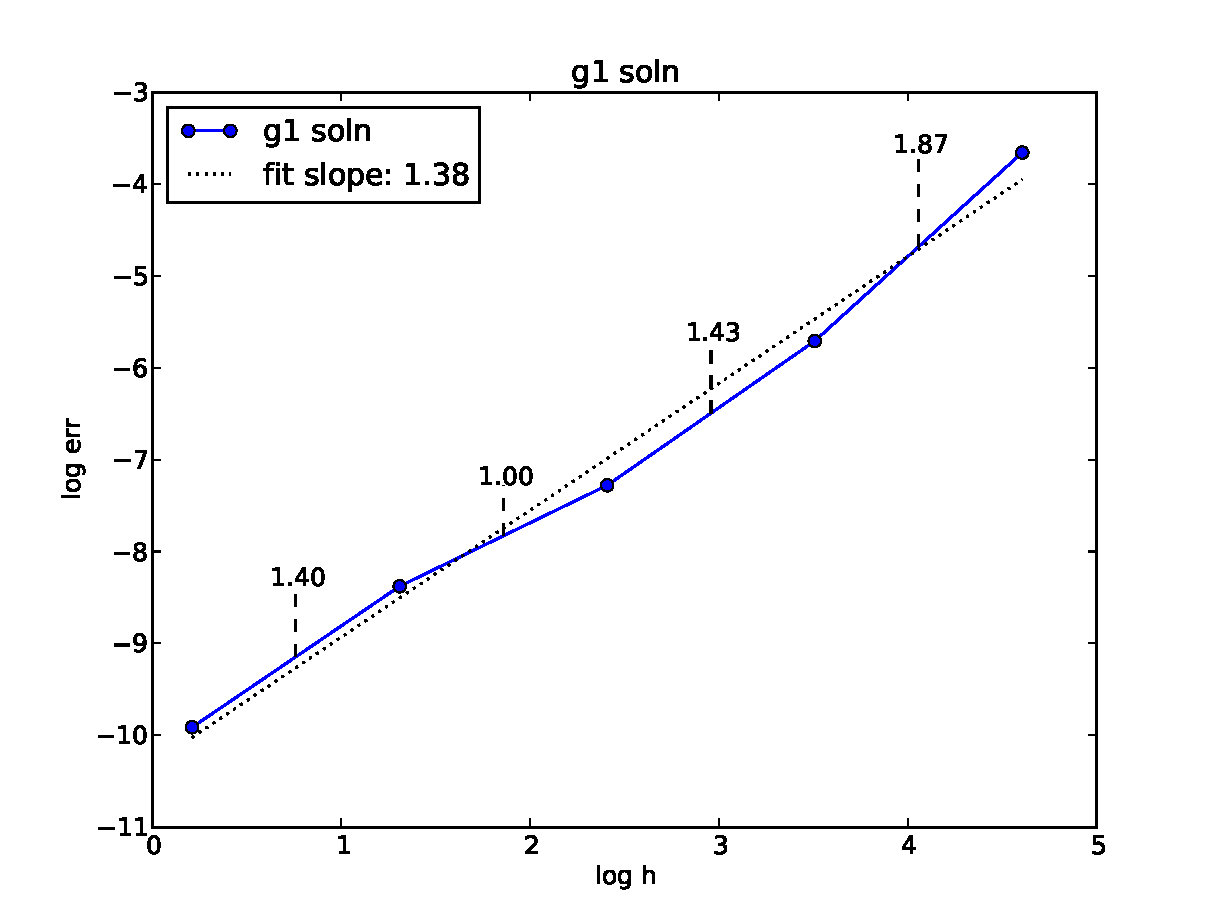
\includegraphics[width=\textwidth]{g1}
%   \caption{$\phi$, Group 1}
%   \label{g1}
%  \end{subfigure}
%  \begin{subfigure}[b]{0.45 \textwidth}
%   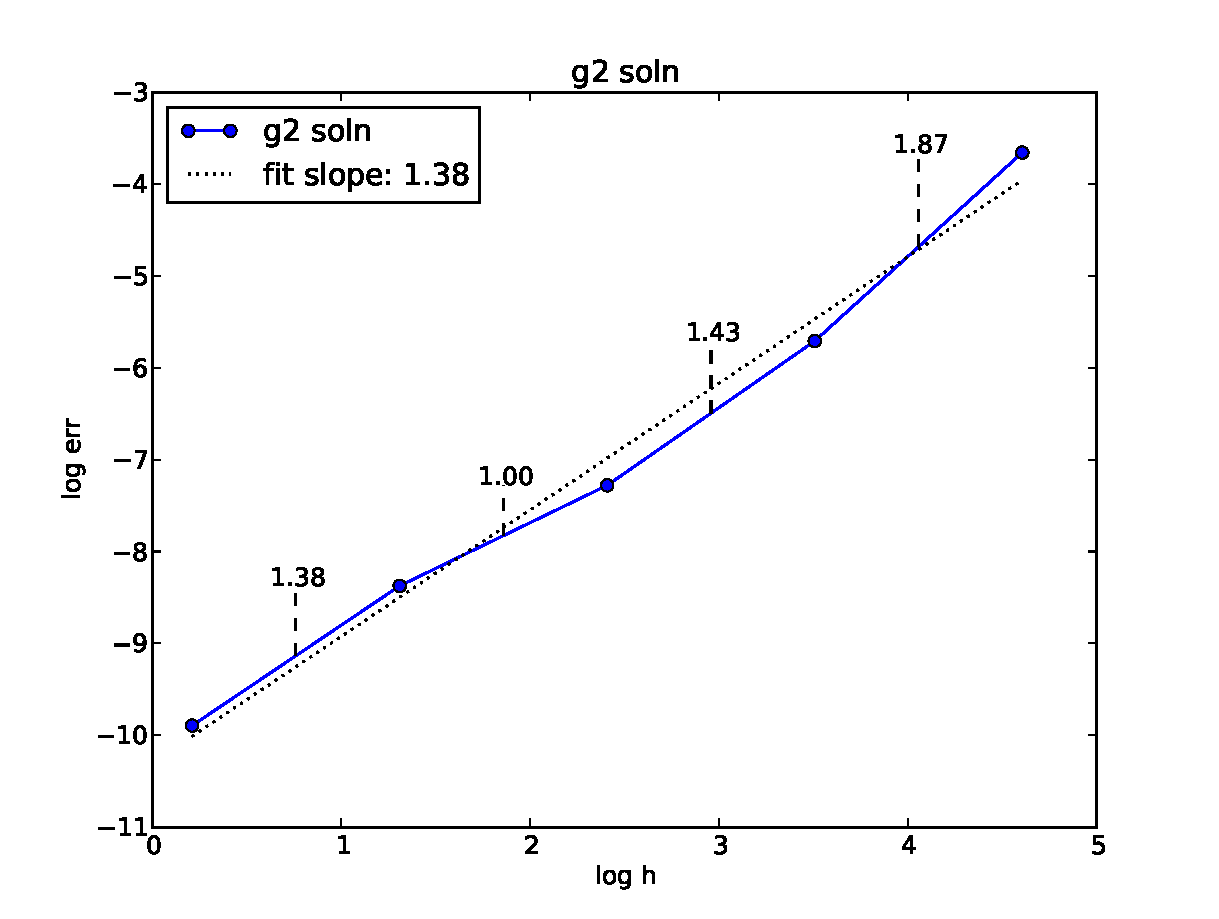
\includegraphics[width=\textwidth]{g2}
%   \caption{$\phi$, Group 2}
%   \label{g2}
%  \end{subfigure}
%  \caption{Spatial Convergence, $\phi$}
%  \label{spatialphi}
%\end{figure}
%\begin{figure}[H]
%\centering
%   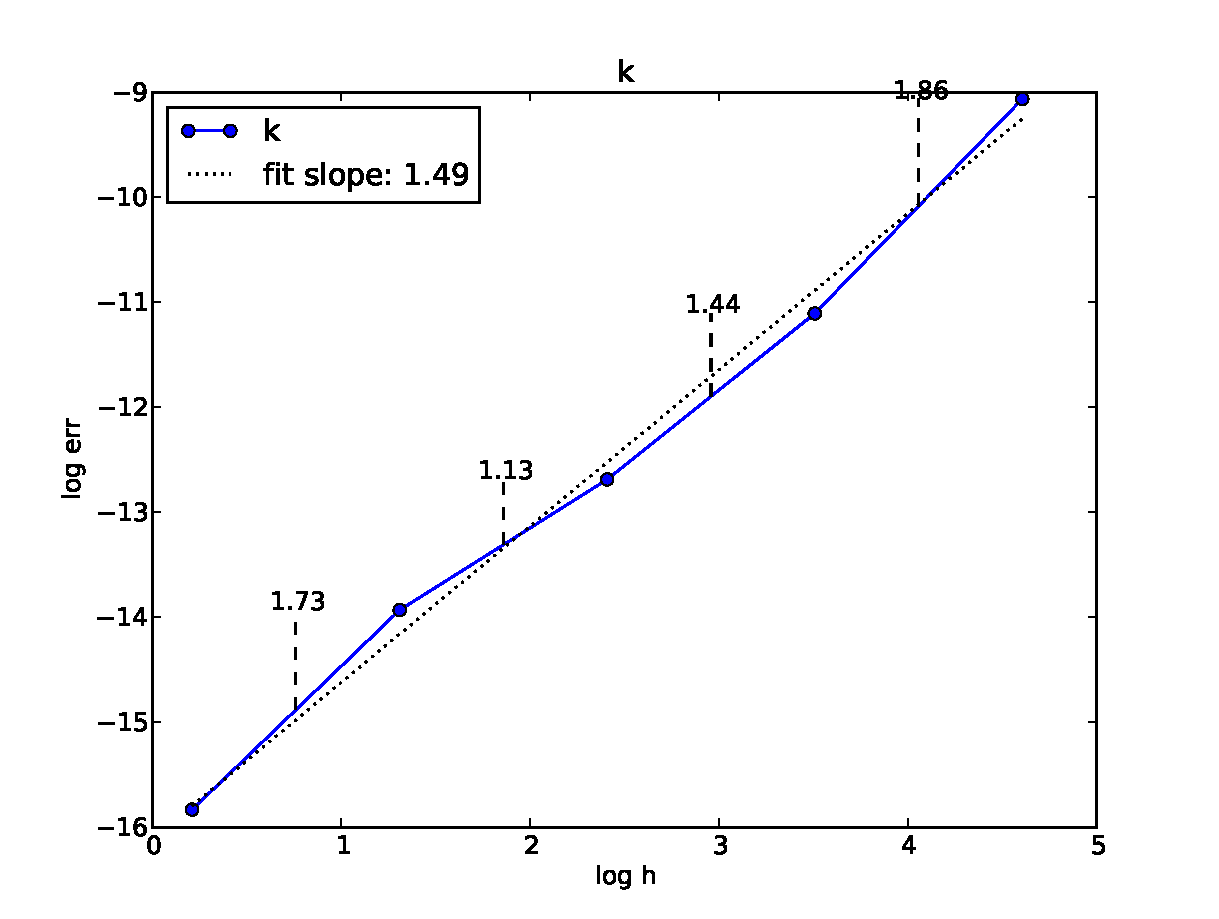
\includegraphics[width=0.5\textwidth]{k}
%   \caption{Spatial Convergence, $k$}
%   \label{spatialk}
%\end{figure}

%\subsection{Stochastic Convergence}
%We vary the number of uncertain inputs including
\begin{table}[H]
\centering
\begin{tabular}{c|c|c}
Material & Property & Distribution \\ \hline
Material 1 & $\nu\Sigma_{2,f}$ & $\mathcal{U}(0.0981,0.1201)$ \\
Material 1 & $\Sigma_{2,c}$ & $\mathcal{U}(0.0499,0.0609)$  \\
Material 4 & $\nu\Sigma_{2,f}$ & $\mathcal{U}(0.0921,0.1121)$ \\
Material 4 & $\Sigma_{2,c}$ & $\mathcal{U}(0.03732,0.04552)$  \\
Material 5 & $D_2$ & $\mathcal{U}(0.1432,0.1752)$ 
\end{tabular}
\caption{Uncertain Input Parameters}
\label{params}
\end{table}

%In order for stochastic collocation to be preferable to Monte Carlo for uncertainty quantification, we desire both the magnitude of the stochastic error to be lower for stochastic collocation, and its convergence rate sufficiently fast to prevent Monte Carlo from being preferable for a given cost (number of PDE solves).
We obtain the error in the moments $r$ of the quantity of interest $k(Y)=u(Y)$, given by
\begin{equation}
\epsilon_h^{(r)}=\frac{|\expv{u_h^{(r)}}-\expv{u_\text{ref}^{(r)}}|}{\expv{u_\text{ref}^{(r)}}},
%S_{N,\Lambda_\text{TD}(L)}[k_h](Y)
\end{equation}
\begin{equation}
\expv{u_h^{(r)}}=\expv{S_{N,\Lambda_\text{TD}(L)}[u_h](Y)^{(r)}}=\sum_{k=1}^\eta w_k ~u_h^{(r)}\qty(Y^{(k)}).
\end{equation}
%where the weights $w_k$ and points $Y^{(k)}$ are the multivariate quadrature used in stochastic collocation.

Figs. \ref{n1mean}-\ref{n5var} show the comparison of Monte Carlo convergence to stochastic collocation for $N=1,3,5$ where $N$ is the number of uncertain parameters.  Both total degree (TD) and hyperbolic cross (HC) index sets have been included for $N>1$ (they are indistinguishable for $N=1$).

Because of the regularity of $k(Y)=u(Y)$, the total degree index set is as cost-effective as the hyperbolic cross index set.  For a less regular stochastic solution, we expect hyperbolic cross would be more efficient.  We also expect the convergence rate to diminish with increasing $N$, and that trend can be seen in the figures for the mean and variance of $k(Y)$. Both the magnitude of the error as well as the convergence rate of stochastic collocation outperforms Monte Carlo for any number of runs.  In addition, heuristic selection of importance weighting improved the accuracy of sparse grid methods by approximately half an order of magnitude.
%\begin{figure}[H]
%\centering
%  \begin{subfigure}[b]{0.24 \textwidth}
%   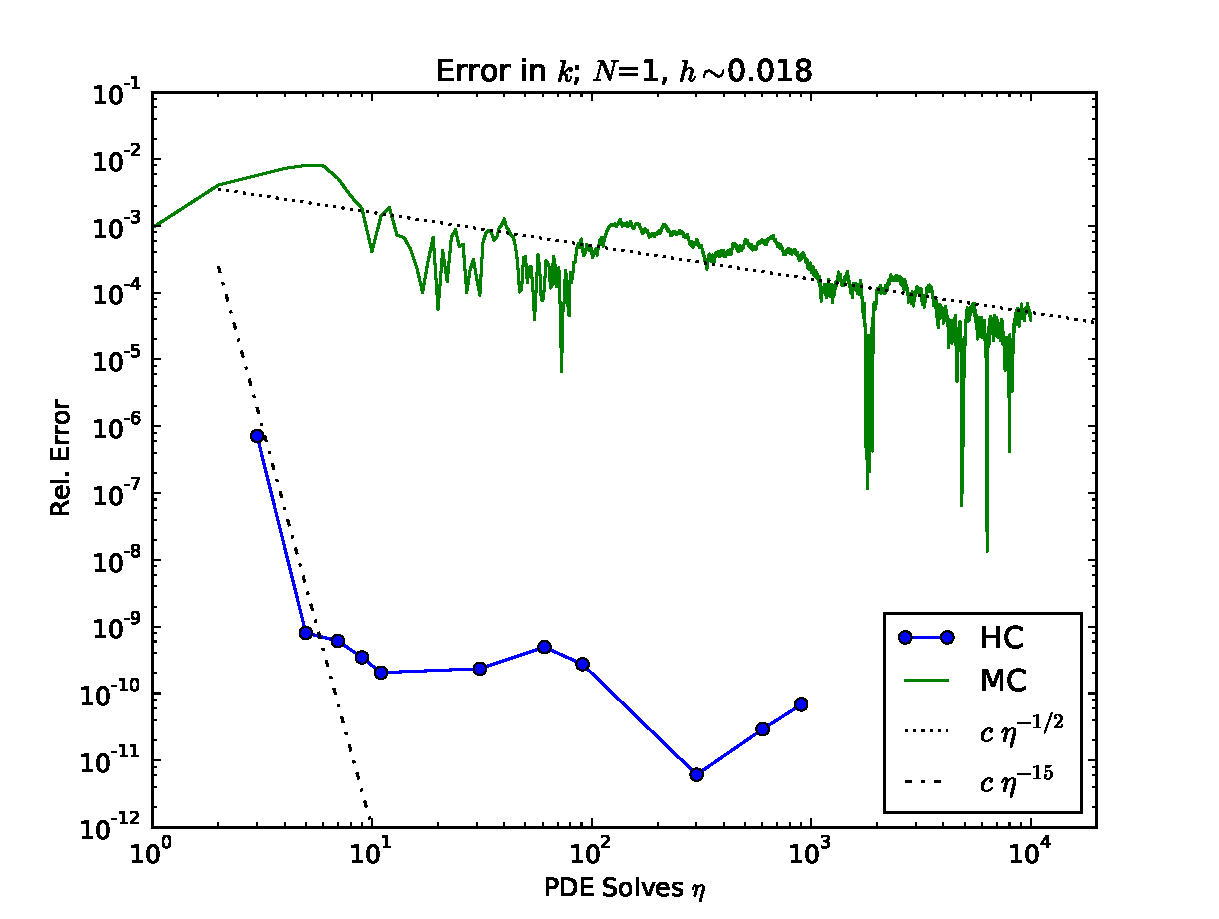
\includegraphics[width=\textwidth]{N1_h5_MCHC}
%   \caption{Mean}
%   \label{n1mean}
%  \end{subfigure}
%  \begin{subfigure}[b]{0.24 \textwidth}
%   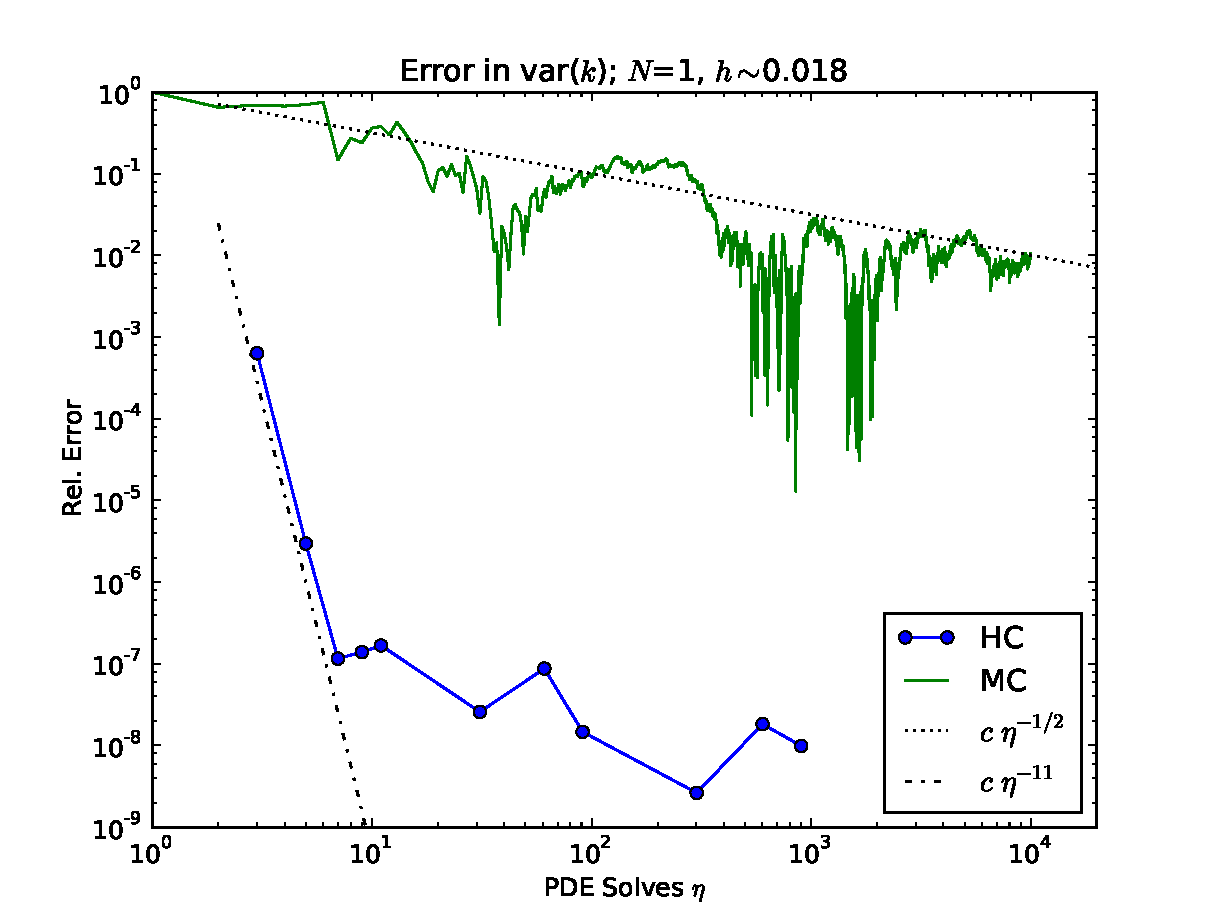
\includegraphics[width=\textwidth]{N1_h5_MCHC_2}
%   \caption{Variance}
%   \label{n1var}
%  \end{subfigure}
%  \caption{$N=1$}
%  \label{n1}
%\end{figure}
%
%\begin{figure}[H]
%\centering
%  \begin{subfigure}[b]{0.24 \textwidth}
%   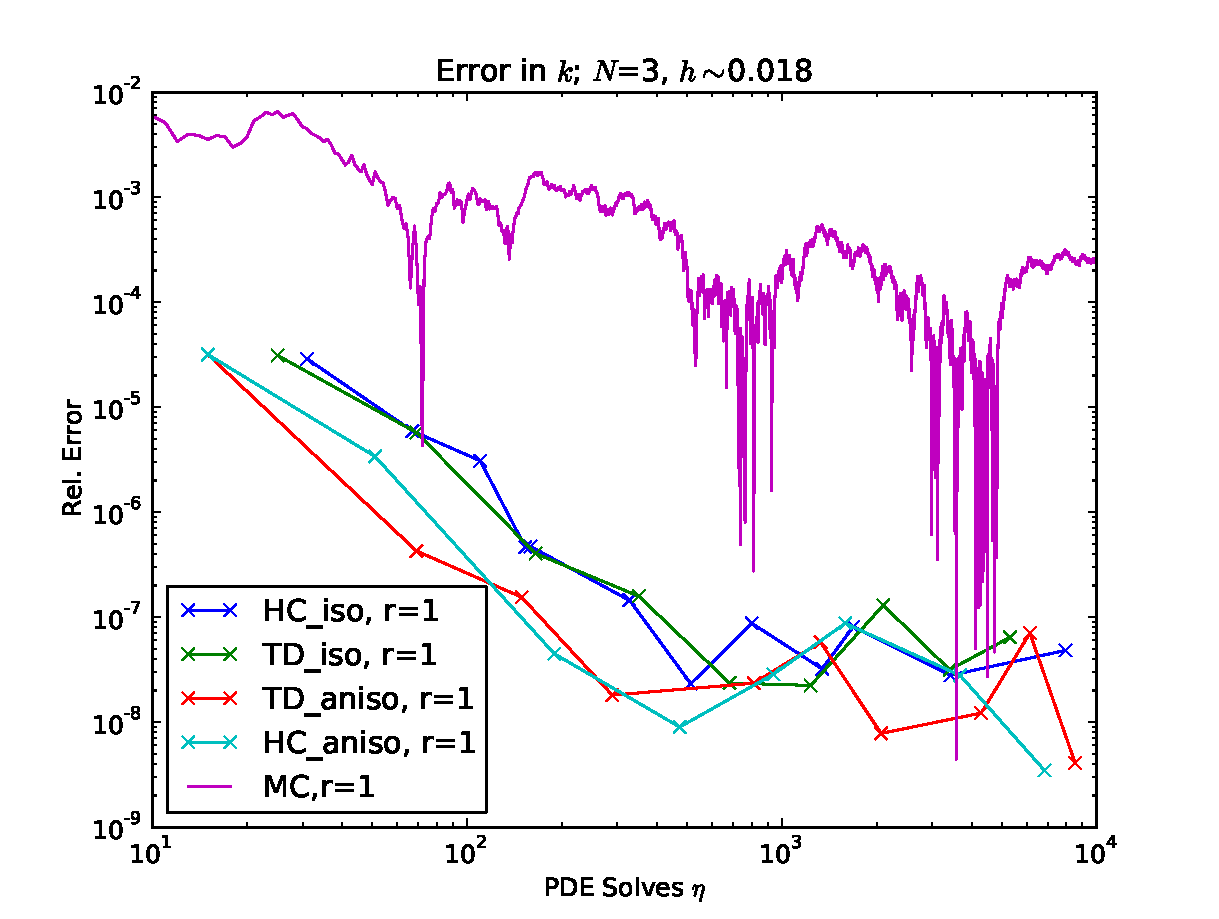
\includegraphics[width=\textwidth]{N3_h5_MCHC}
%   \caption{Mean}
%   \label{n3mean}
%  \end{subfigure}
%  \begin{subfigure}[b]{0.24 \textwidth}
%   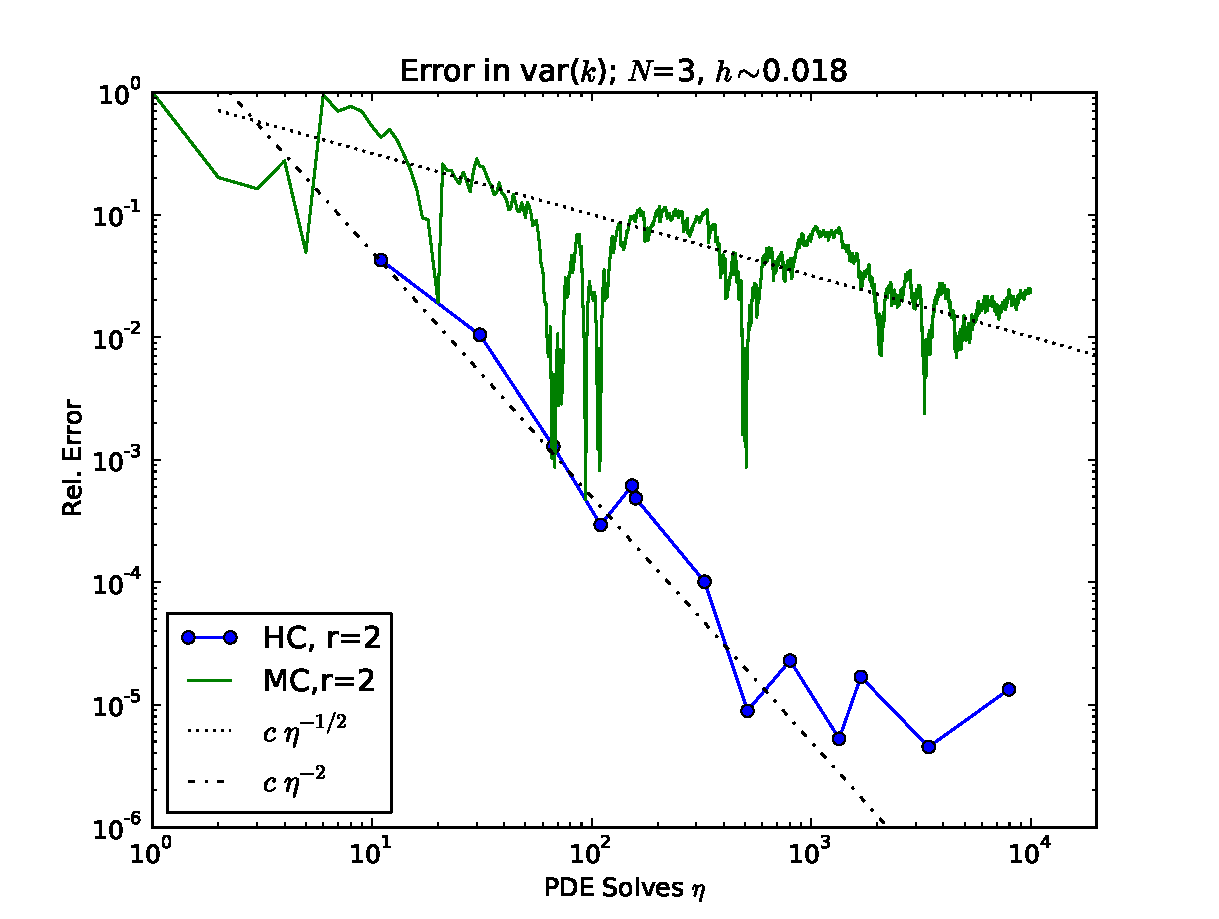
\includegraphics[width=\textwidth]{N3_h5_MCHC_2}
%   \caption{Variance}
%   \label{n3var}
%  \end{subfigure}
%  \caption{$N=3$}
%  \label{n3}
%\end{figure}
%
%\begin{figure}[H]
%\centering
%  \begin{subfigure}[b]{0.24 \textwidth}
%   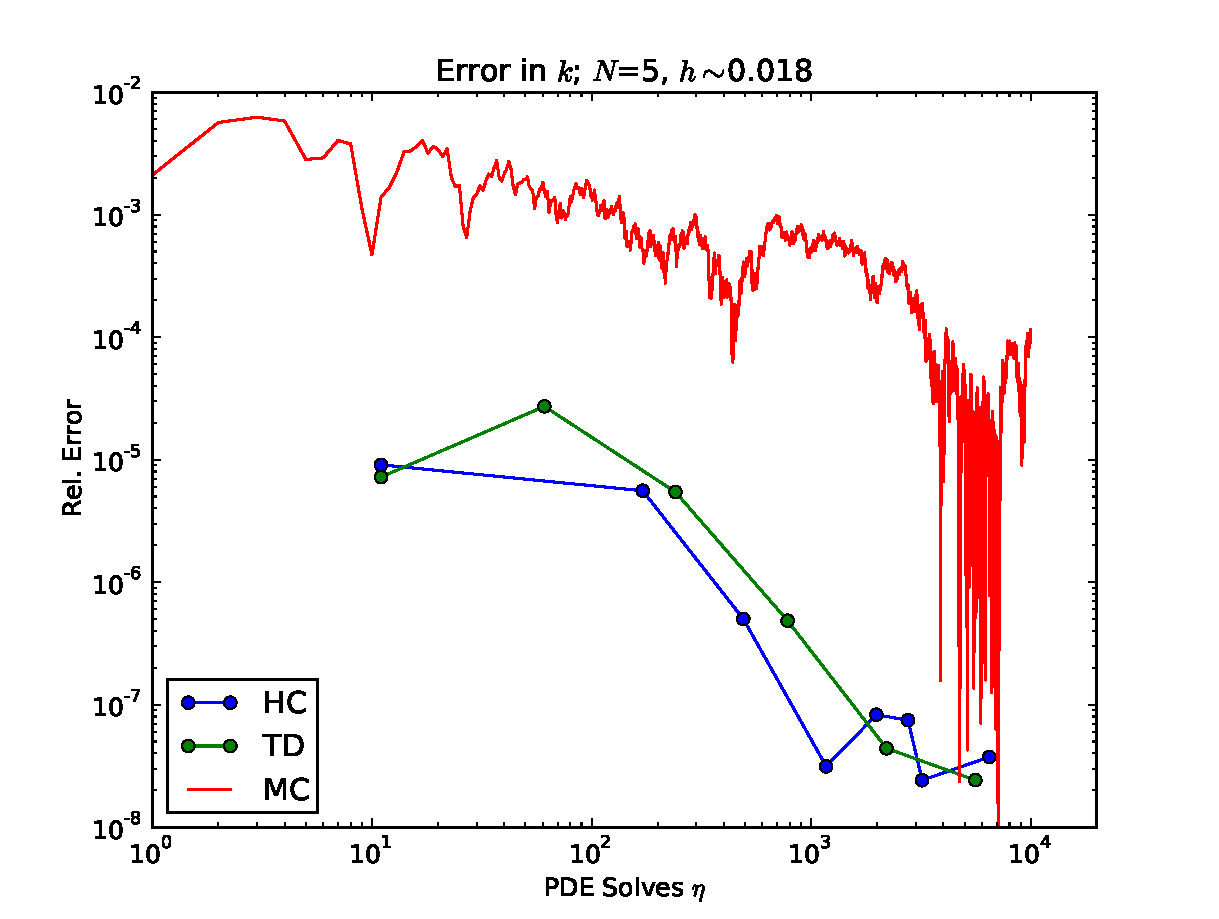
\includegraphics[width=\textwidth]{N5_h5_MCHC}
%   \caption{Mean}
%   \label{n5mean}
%  \end{subfigure}
%  \begin{subfigure}[b]{0.24 \textwidth}
%   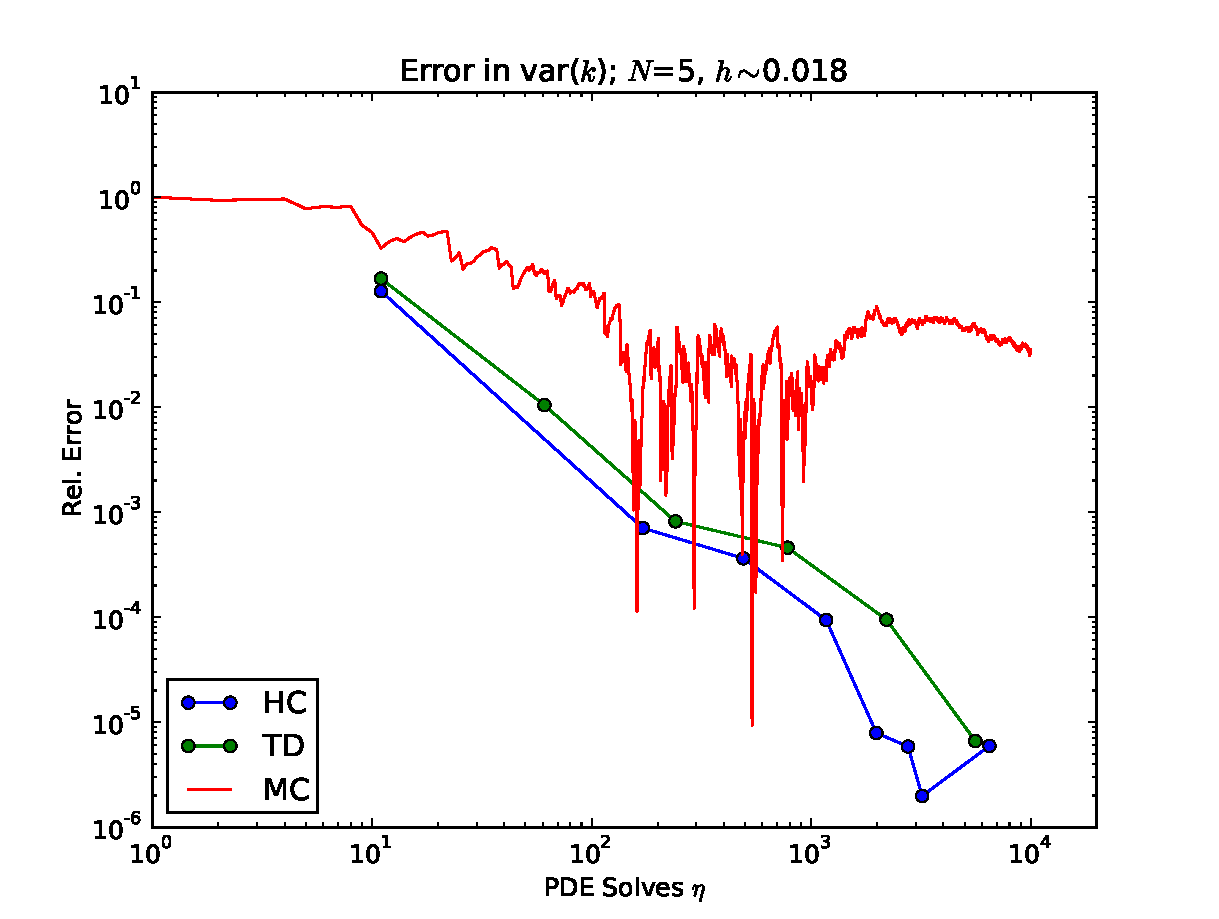
\includegraphics[width=\textwidth]{N5_h5_MCHC_2}
%   \caption{Variance}
%   \label{n5var}
%  \end{subfigure}
%  \caption{$N=5$}
%  \label{n5}
%\end{figure}
%  \begin{figure}[H]
%   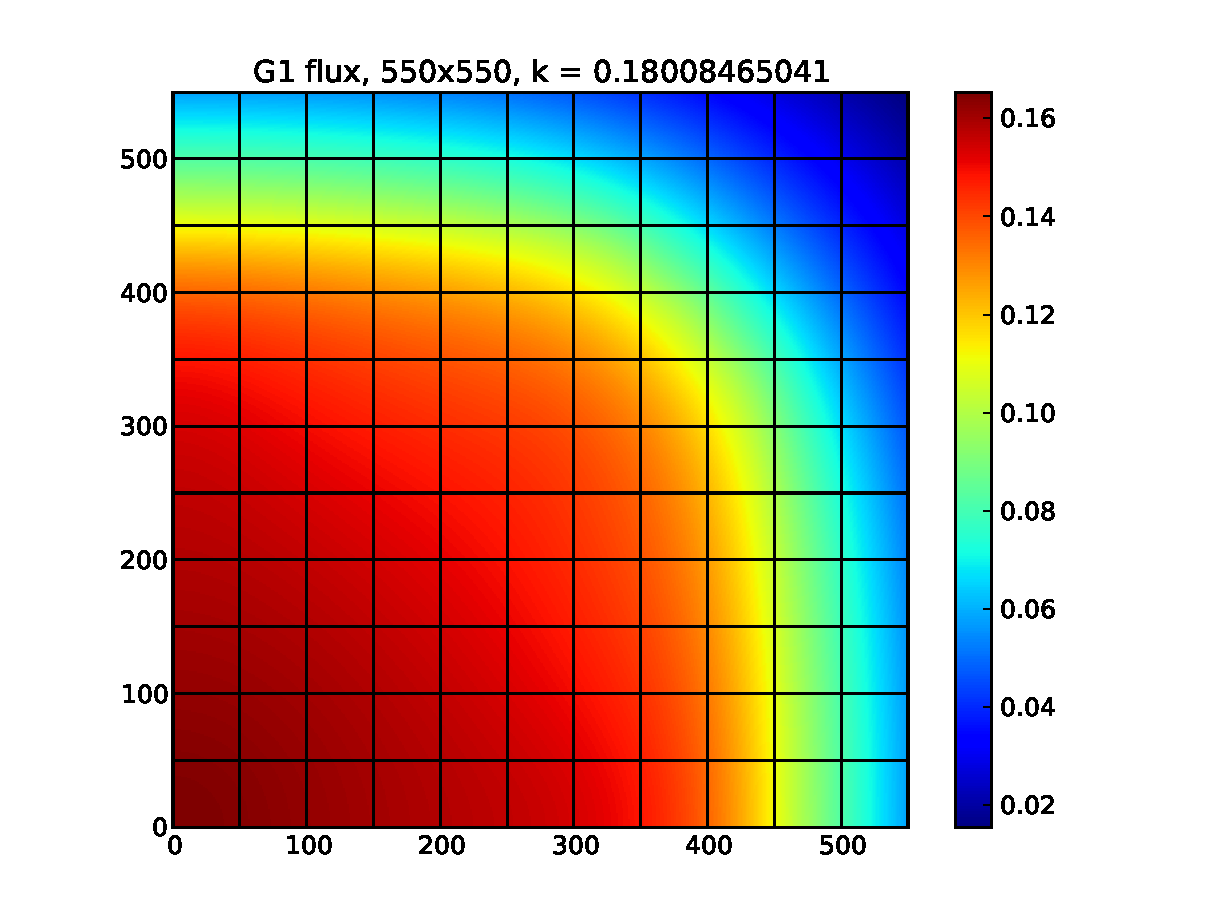
\includegraphics[width=0.45\textwidth]{g1_50_flux}
%   \caption{$N=1$, PLACEHOLDER pdf}
%   \label{kpdf_1}
%  \end{figure}
%  \begin{figure}[H]
%   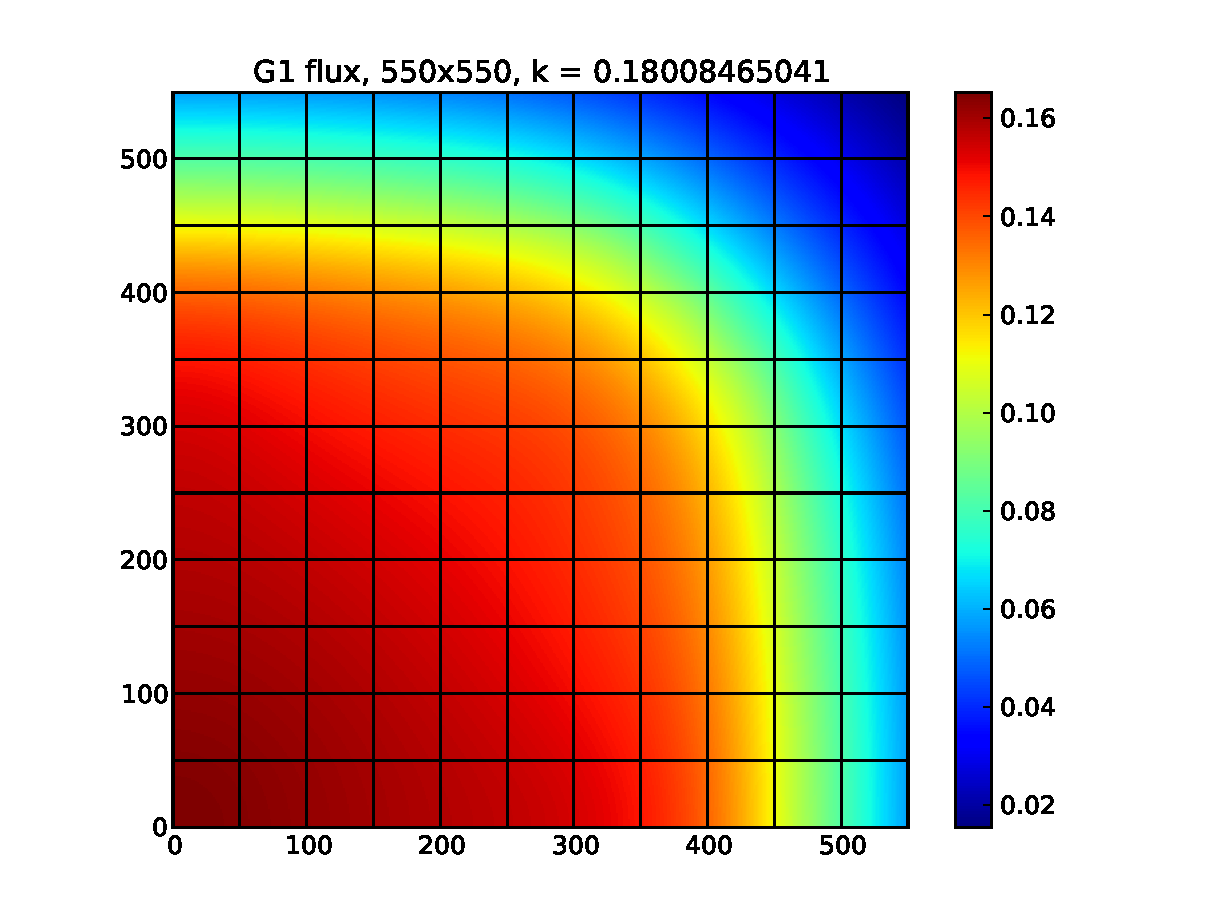
\includegraphics[width=0.45\textwidth]{g1_50_flux}
%   \caption{$N=3$, PLACEHOLDER pdf}
%   \label{kpdf_3}
%  \end{figure}
%    \begin{figure}[H]
%   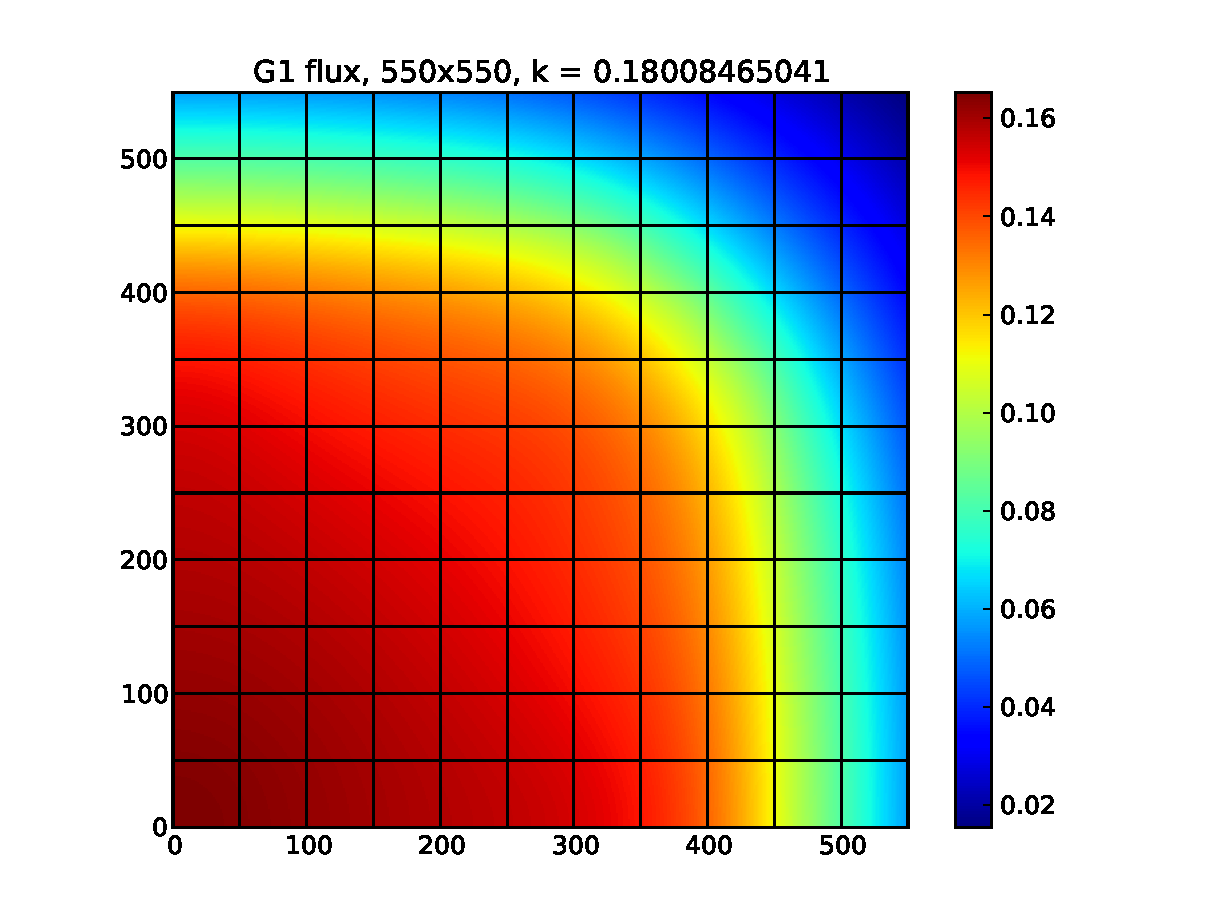
\includegraphics[width=0.45\textwidth]{g1_50_flux}
%   \caption{$N=5$, PLACEHOLDER pdf}
%   \label{kpdf_5}
%  \end{figure}
  
  \begin{figure}[htb]
   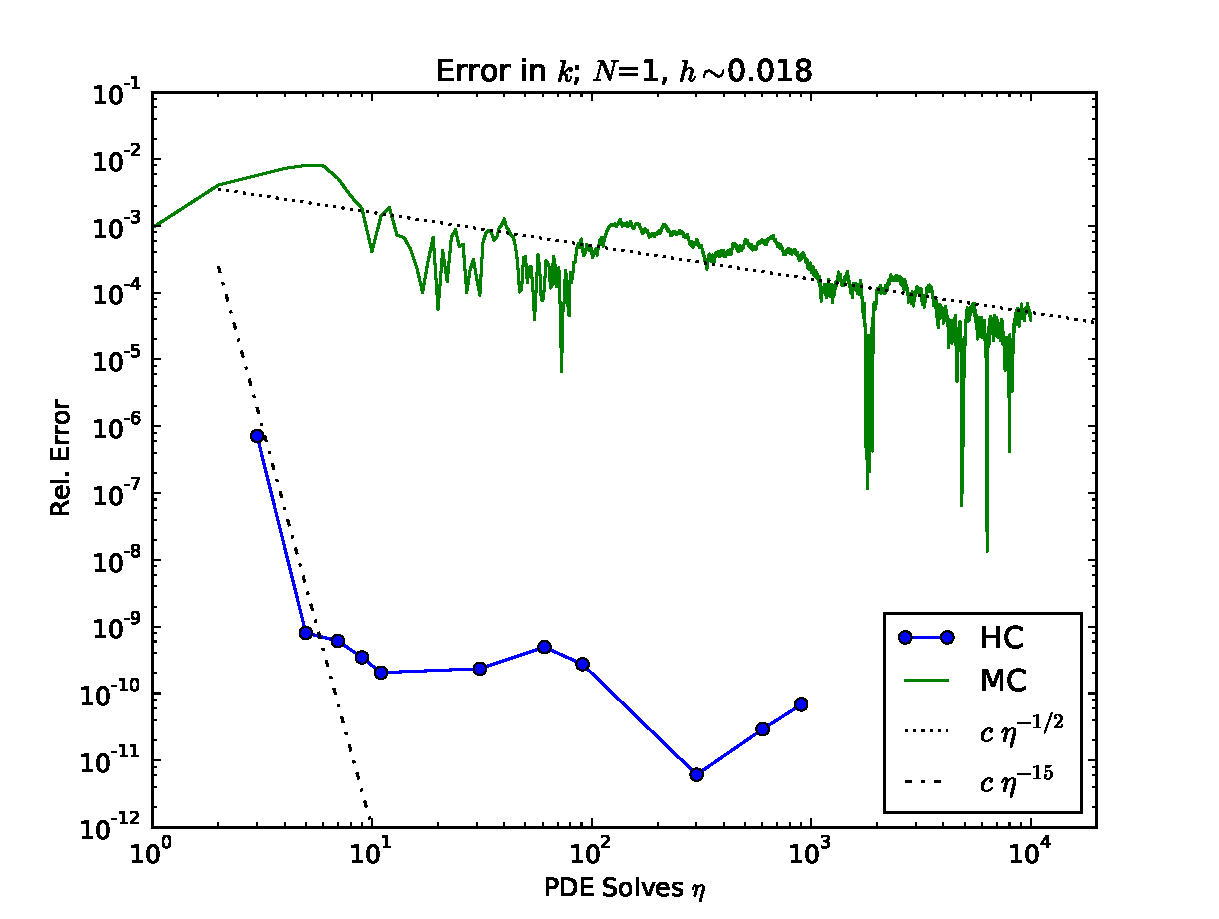
\includegraphics[width=0.45\textwidth]{N1_h5_MCHC}
   \caption{$N=1$, Mean}
   \label{n1mean}
  \end{figure}
  \begin{figure}[htb]
   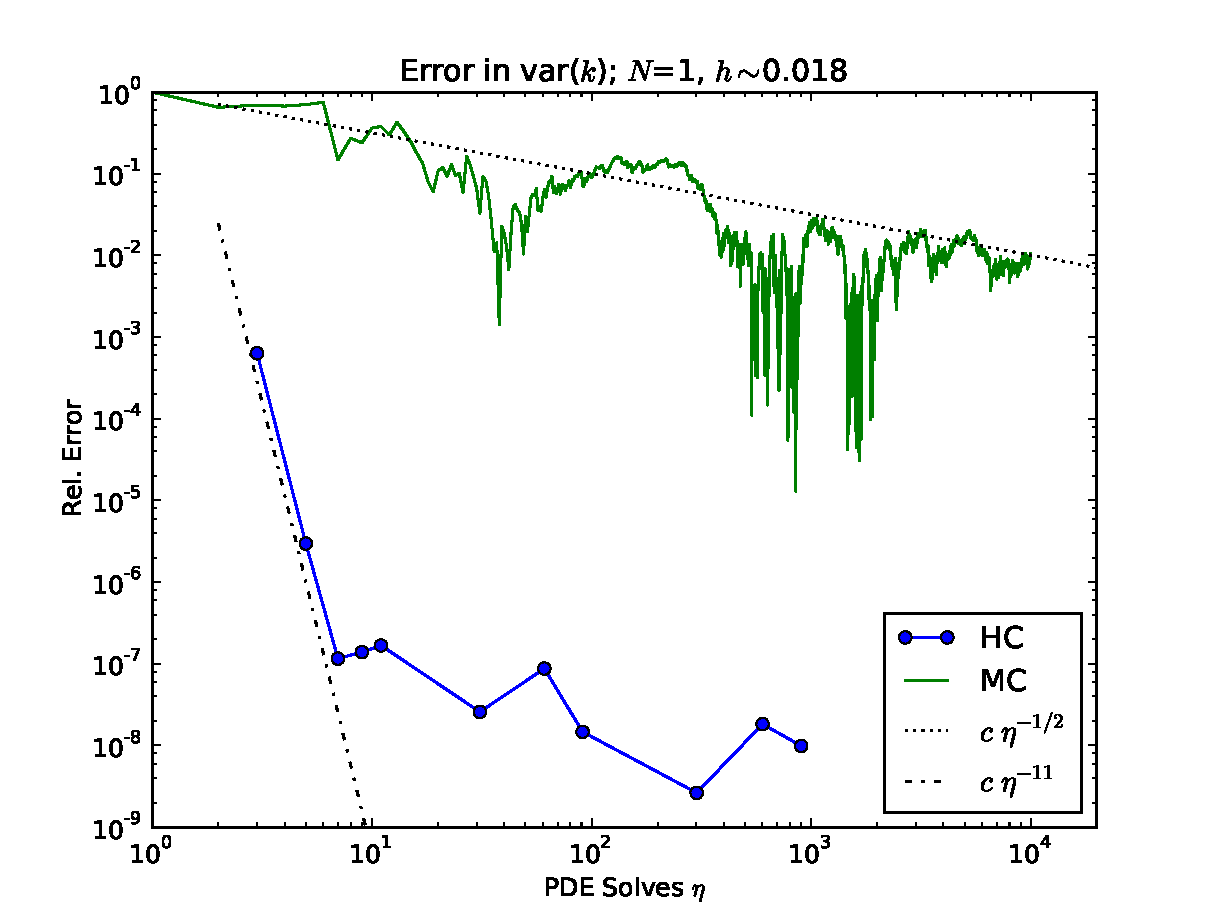
\includegraphics[width=0.45\textwidth]{N1_h5_MCHC_2}
   \caption{$N=1$, Variance}
   \label{n1var}
  \end{figure}

  \begin{figure}[htb]
   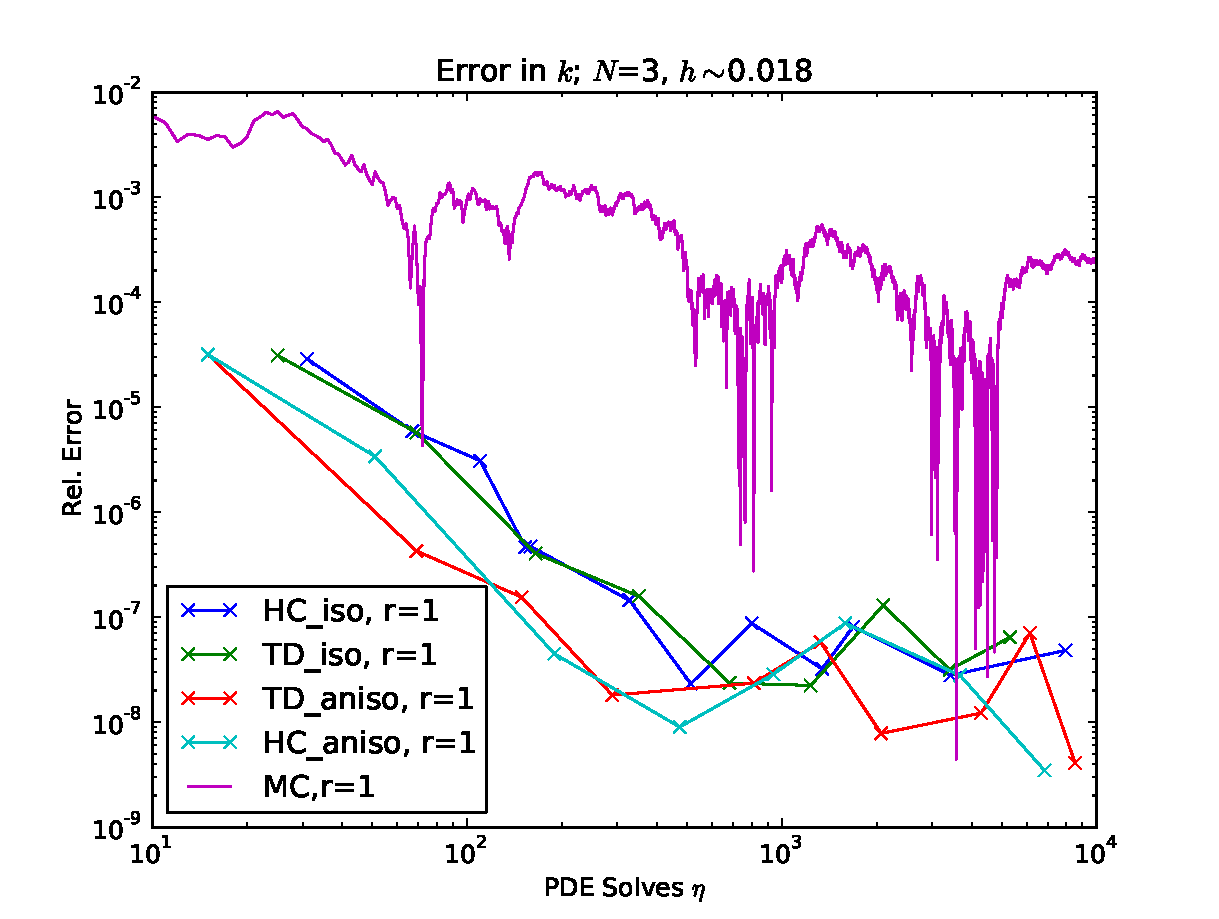
\includegraphics[width=0.45\textwidth]{N3_h5_MCHC}
   \caption{$N=3$, Mean}
   \label{n3mean}
  \end{figure}
  \begin{figure}[htb]
   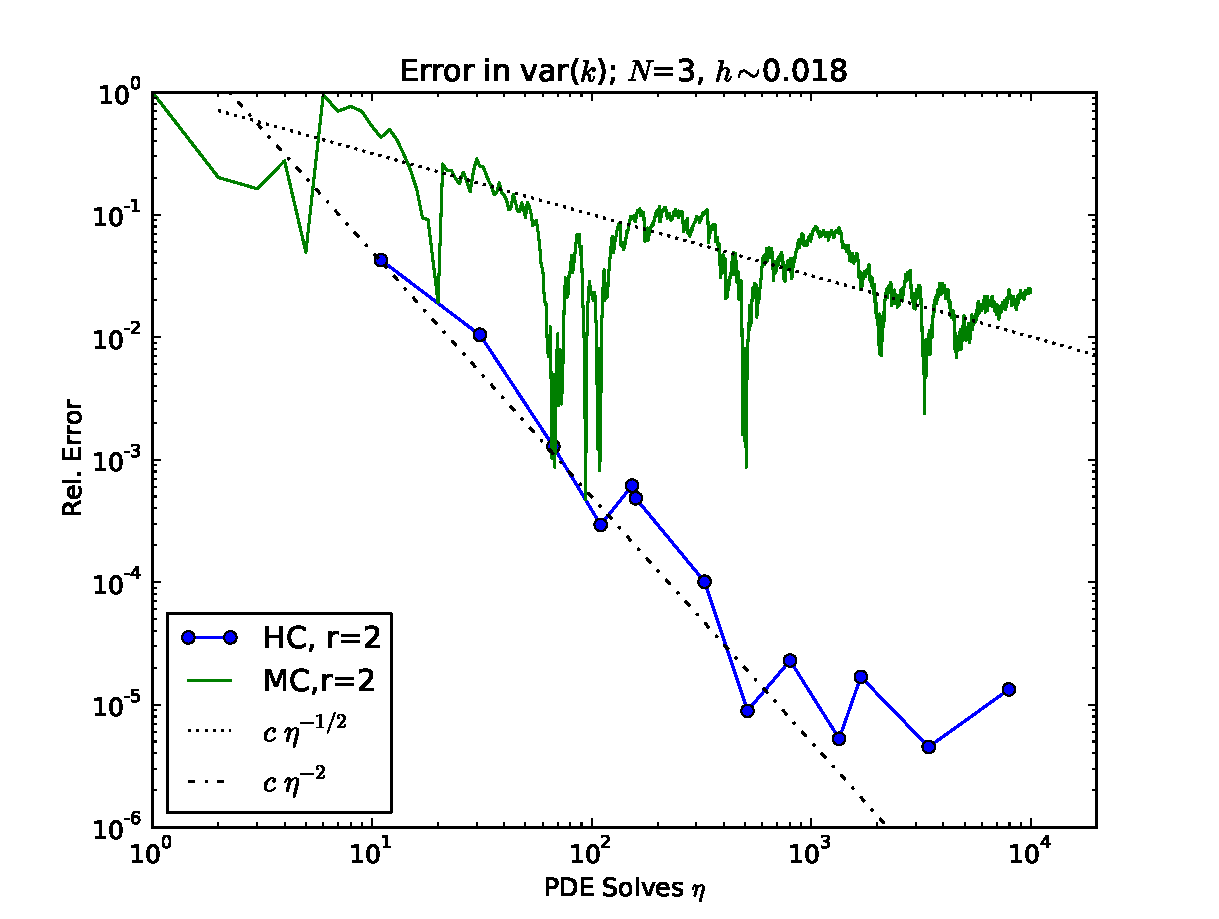
\includegraphics[width=0.45\textwidth]{N3_h5_MCHC_2}
   \caption{$N=3$, Variance}
   \label{n3var}
  \end{figure}


  \begin{figure}[htb]
   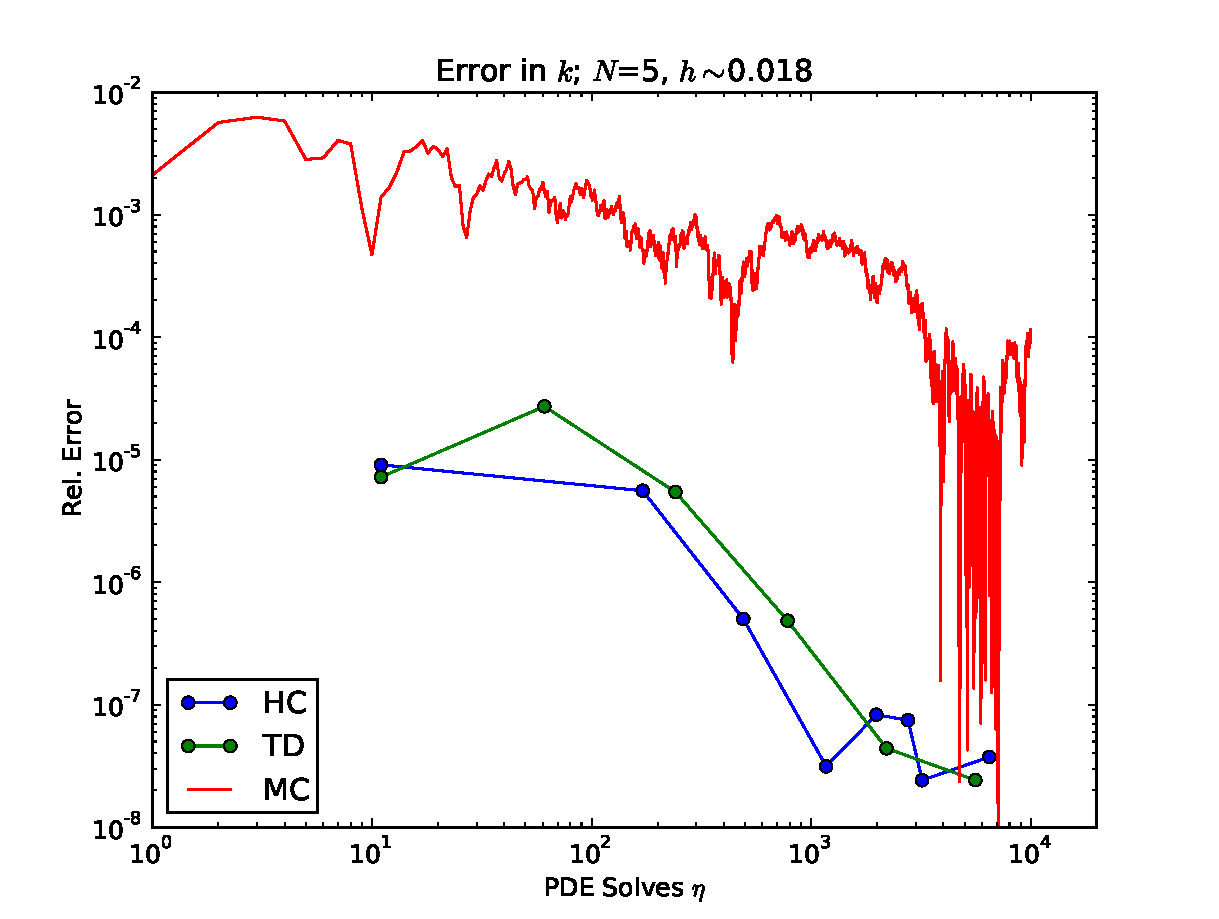
\includegraphics[width=0.45\textwidth]{N5_h5_MCHC}
   \caption{$N=5$, Mean}
   \label{n5mean}
  \end{figure}
  \begin{figure}[htb]
   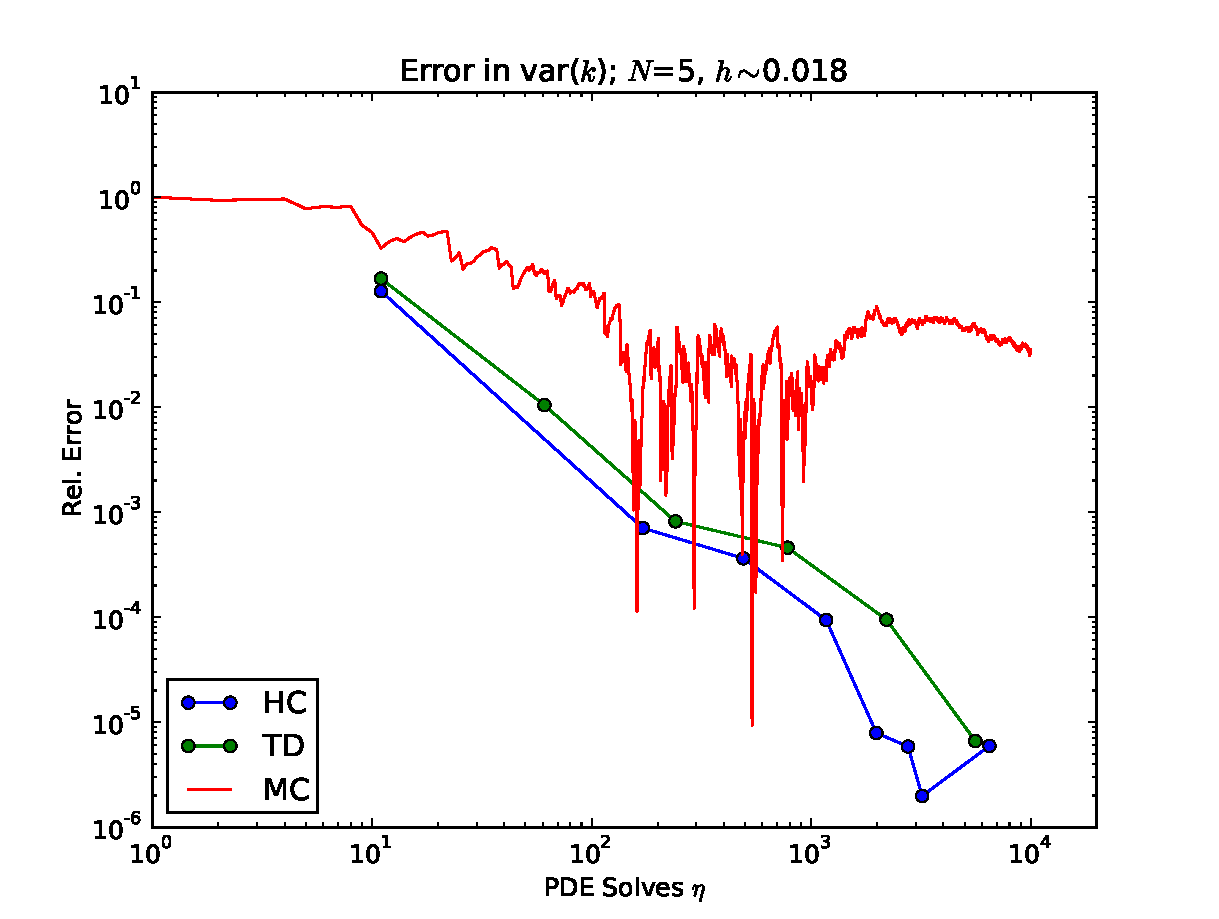
\includegraphics[width=0.45\textwidth]{N5_h5_MCHC_2}
   \caption{$N=5$, Variance}
   \label{n5var}
  \end{figure}
  
\subsection{Anisotropic Sparse Grid}
We present four sets of importance choices and the effect on absolute error and convergence, along with Monte Carlo and isotropic sparse grids.  Each case is labeled by its importance weights in order of the input parameters listed in Table \ref{params}, each considering $N=5$ uncertain inputs. The choice of weights is informed by considering the convergence rate varying each individual parameter alone.  We choose the sample cases $\alpha=(1,1,2,2,4)$ and $\alpha=(1,1,4,4,8)$ to put increasing weight on the material 1 cross sections and remove weight from the material 5 diffusion coefficient.  In addition, we intentionally choose a poor weighting scheme with $\alpha=(4,4,2,2,1)$ to show worst-case effects of including importance weights.  The results are compared in Figs. \ref{aniso1} and \ref{aniso2} for the mean and variance. 
%\begin{figure}[H]
%\centering
%   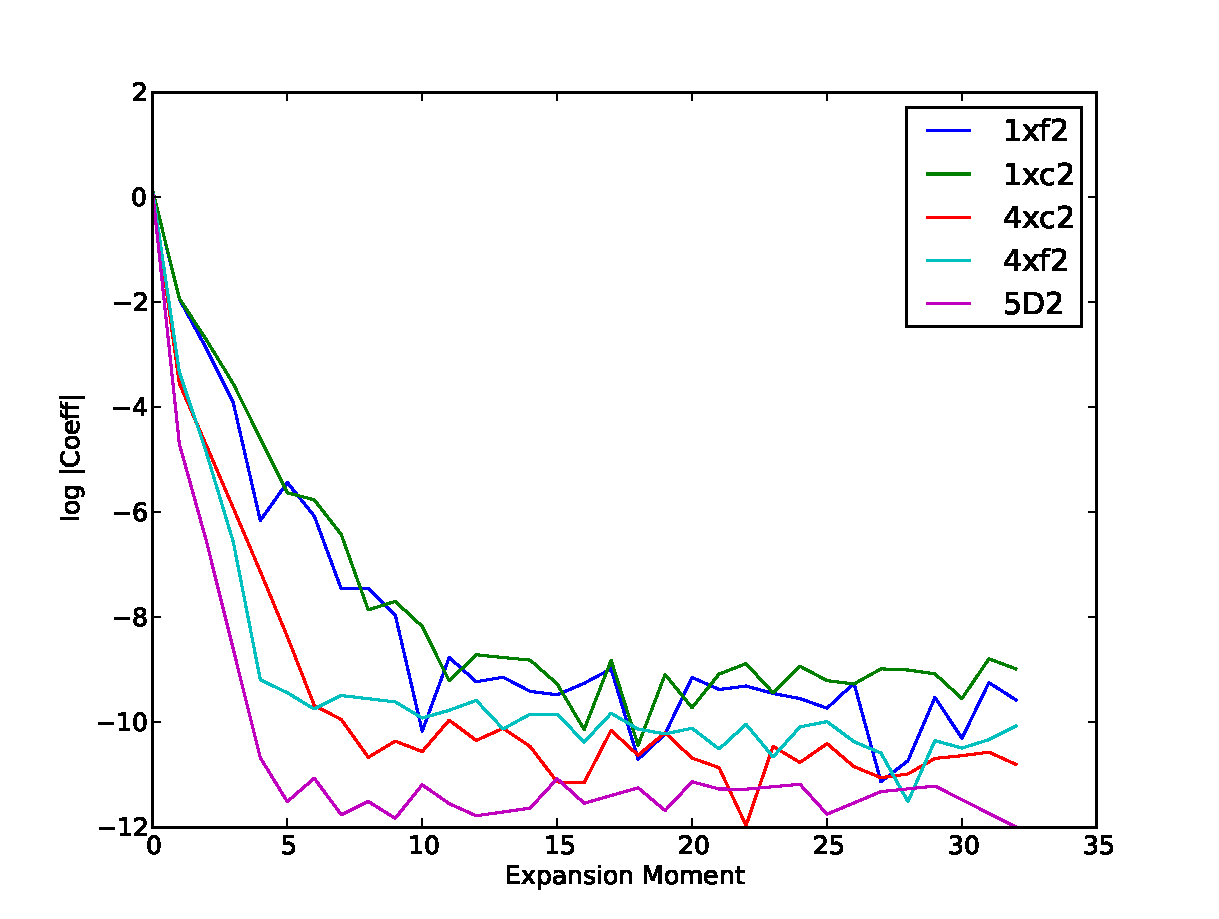
\includegraphics[width=0.45\textwidth]{coefficient_decay2}
%   \caption{Independent Stochastic Convergence}
%   \label{indconv}
%\end{figure}

  \begin{figure}[htb]
   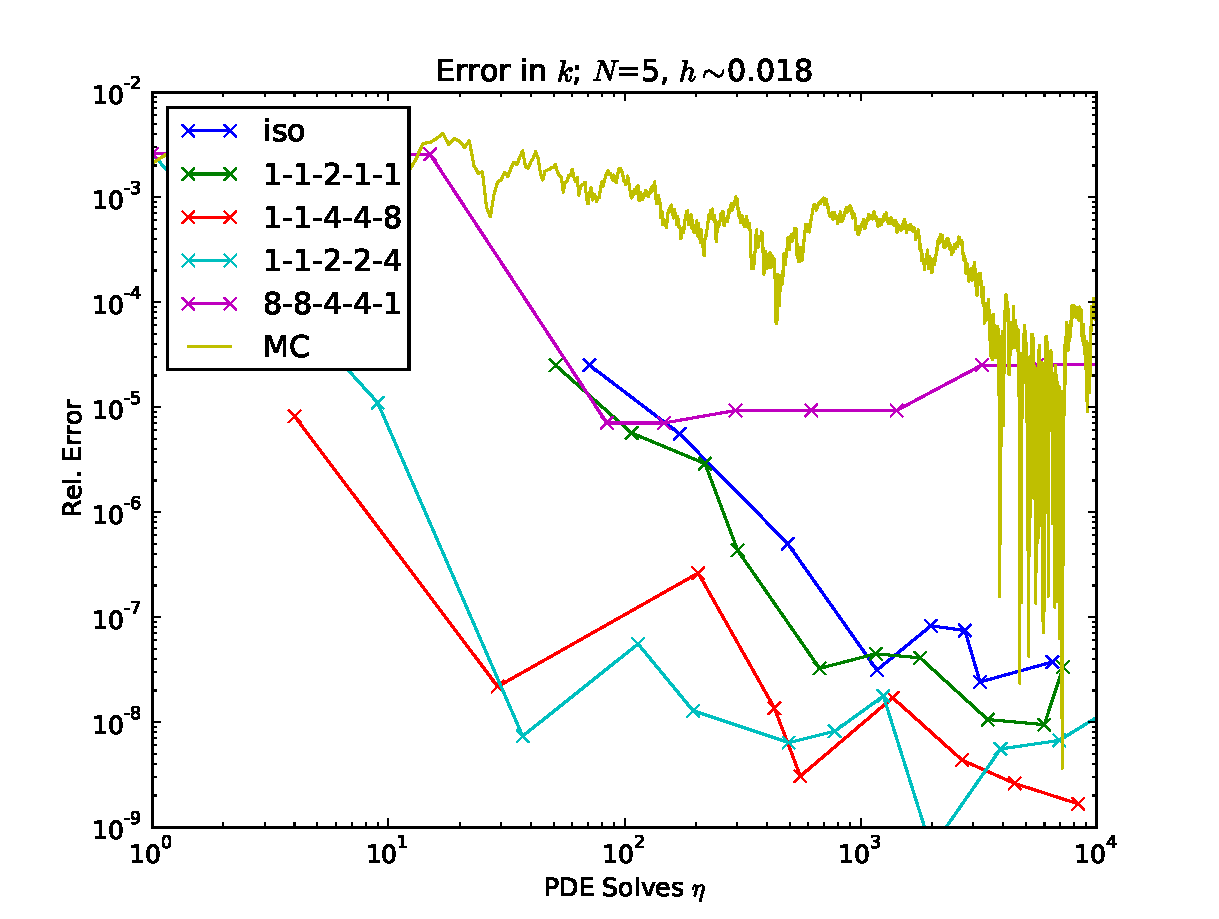
\includegraphics[width=0.45\textwidth]{N5_h5_aniso1}
   \caption{Anisotropic, Mean}
   \label{aniso1}
  \end{figure}
  \begin{figure}[htb]
   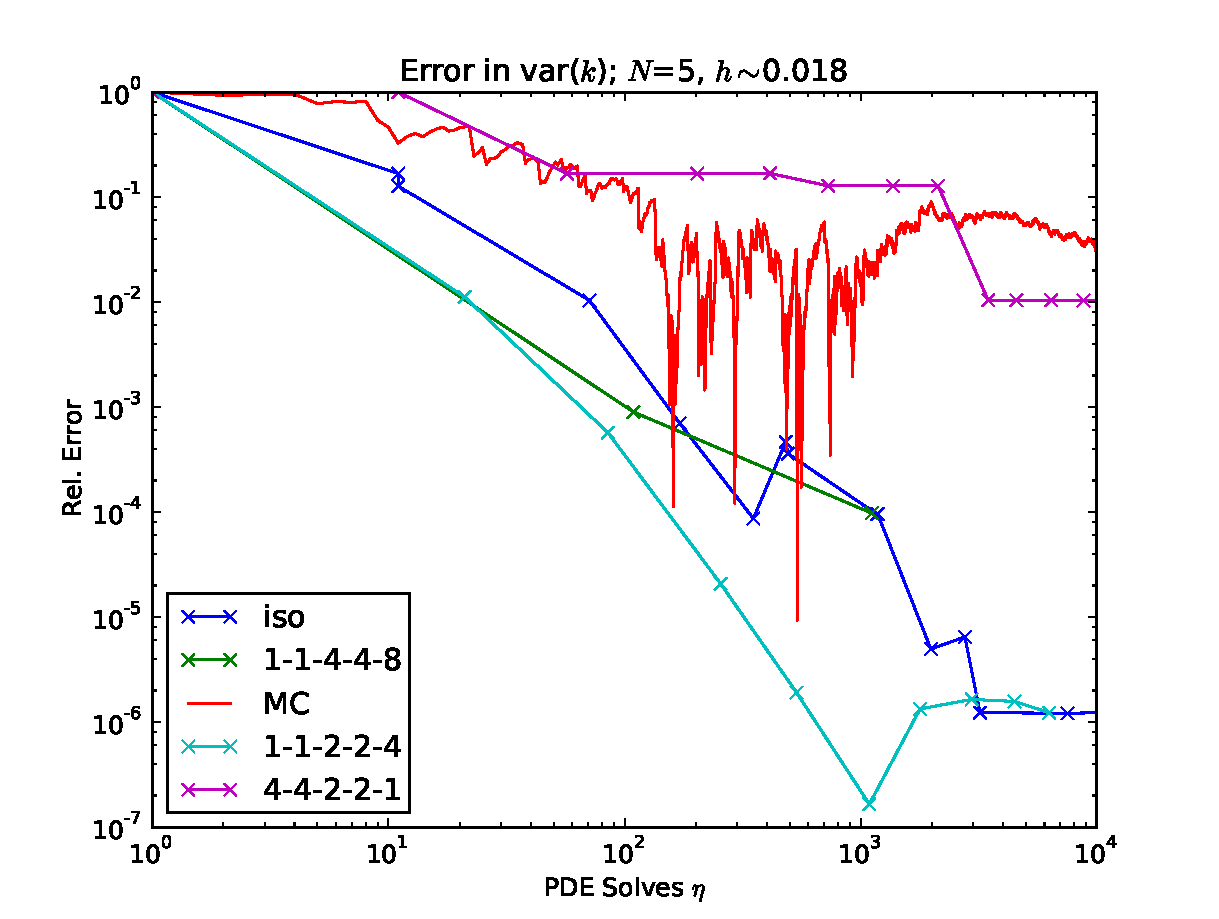
\includegraphics[width=0.45\textwidth]{N5_h5_aniso2}
   \caption{Anisotropic, Variance}
   \label{aniso2}
  \end{figure}



\section{Discussion}
We make a few considerations in analyzing our results.
First, there is a correlation between the iterative tolerance of the deterministic solver and the maximum convergence of uncertainty quantification.  If the deterministic space is poorly resolved, it limits the possible convergence in stochastic space.
%First, there is a noticeable plateau in error convergence in many of the stochastic collocation plots.  This seems to be an artifact of the algorithm, which uses an iterative tolerance of $\Delta k <1\times10^{-6}$.  Because the deterministic solver is only accurate to 6 orders of magnitude, the accuracy of the stochastic solver is limited by this value.  We expect reducing the deterministic tolerance to result in further possible convergence in stochastic space. 

Additionally, the number of PDE solves for stochastic collocation is determined based on the maximum expansion level $L$.  For higher $N$, increasing $L$ by only one value increases the number of PDE solves much more than increasing $L$ by one for small $N$.  As a result, there are few data points to power fit for $N=5$, and the plateau just mentioned around $\epsilon=10^{-8}$ is more difficult to distinguish from standard convergence.  Resolving the issues leading to the plateau should also resolve this difficulty in fitting points.

We can see the possible benefit and harm of applying importance weighting to an anisotropic grid in Figs. \ref{aniso1} and \ref{aniso2}.  Any application of anisotropic sparse grids in line with our heuristic assessment significantly improves the magnitude of error for a given number of PDE solves.  We note, however, that the convergence of $\alpha=(1,1,2,2,4)$ is better than the more extreme $\alpha=(1,1,4,4,8)$.  This suggests that with $\alpha=(1,1,2,2,4)$ we have achieved an optimum efficiency that isn't improved with further anisotropy.  However, the anisotropy intentionally chosen poorly, $\alpha=(4,4,2,2,1)$, shows much worse convergence than the isotropic case, and for the variance is on par with Monte Carlo.
Given these limitations, it is clear that for the uncertain spaces presented, stochastic collocation shows much better convergence and magnitude of error for the same cost when compared with Monte Carlo. 

%\section{Ongoing Work}
%The work presented here considers a maximum number of uncertain variables $N=5$.  While demonstrative of expected savings for larger input spaces, showing the convergence rates of isotropic and anisotropic sparse grids for large $N$ is desirable.  We expect to see diminishing returns in using stochastic collocation as the input space grows in dimensionality.\\
%
%One effective method for very large numbers of uncertain inputs is HDMR, which uses sets of low-order stochastic interactions between a few variables at a time to approximate the full stochastic problem.  In the event the number of uncertain parameters becomes very large, HDMR could prove less costly than stochastic collocation for many problems. \\
%
%Lastly, our work so far has been demonstrated exclusively with uniformly-distributed random variables as input parameters.  To more accurately approximate the shape of an arbitrary probability distribution, we intend to implement Beta-distributed random variables using Jacobi quadrature, with two shaping parameters $\alpha,\beta$.  The Beta distribution is also distributed finitely between two points, but $\alpha,\beta$ can be adjusted to accommodate a wide range of uncertain distributions including uniform and truncated Gaussian normal distributions.  While Beta distributions cannot exactly replicate all other distributions, we expect it can replicate them without introducing a greater error than introduced by the Monte Carlo and stochastic collocation methods presented.

%\newpage
\bibliography{uq}{}
\bibliographystyle{plain}
\end{document}